% !TEX root = ../thesis.tex
\chapter{Experimente} % (fold)
\label{cha:experimente}
\section{Tracking}

Für das Approximieren von Parametern anhand von realen Daten wird ein geeigneter Datensatz benötigt.
Insbesondere werden die Trajektorien der Fische benötigt. Fische haben hierbei den Vorteil, dass sie pseudo-dreidimensional sind. Werden die Schwärme in einem relativ niedrigen Becken gehalten, so kann sich auf deren X und Y Komponente beschränkt werden. Natürlich existiert hierbei die Z-Komponente, welche aber durch das flache Becken keine große Ausprägung erfährt. Eine Konsequenz einer existierenden Z-Komponente ist, dass Fische sich überlagern können und dadurch die Problematik entsteht, diese im Prozess des Trackens trennen zu müssen. Ein weiterer Vorteil ist, dass das Tracken von Schwärmen, deren Z-Komponente nicht vernachlässigbar ist, ein wesentlich komplexeres Unterfangen ist. Betrachtet man einen Vogelschwarm, so muss dieser mit zwei kalibrierten Kameras aufgenommen werden.
Hieraus resultieren Aufnahmen des Vogelschwarms, welche auf zwei Ebenen aufgeteilt sind (Beispielsweise die XY und XZ-Ebene). Um daraus die dreidimensionalen Positionen der Vögel zu extrahieren, müssen diese Ebenen registriert werden, was Material für eine eigenständige Masterthesis liefert. Des Weiteren besteht das Problem, dass sich der Schwarm als Ganzes im Raum bewegt, die Kameras jedoch stationär sind. Eventuell fliegen einzelne Individuen weit genug weg, um von der Kamera nicht erfasst werden zu können. Aus den genannten Gründen wird sich im weiteren Verlauf auf die Trajektorien von Fischen beschränkt.

Es wird ein Datensatz, welcher aus Aufnahmen von Fischschwärmen der Spezies \textit{juvenile zebrafish} besteht, verwendet. Die Größe eines ausgewachsenen Zebrafisches liegt zwischen 10.0 und 19.5 mm. Die Videos der Schwärme wurden mit einer Auflösung von 3712 x 3740 Pixeln aufgenommen. Die Bildrate beträgt 32 Bilder Pro Sekunde. Die verwendete Kamera ist eine \textit{Emergent Vision HT-20000M} welche mittig 70mm über dem Fischbecken montiert ist.
Das kreisförmige Fischbecken ist gefüllt mit 28 Grad warmen Wasser, welches der benötigten Wassertemperatur der Zebrafische entspricht. Die Wassertiefe beträgt 2,5 cm und der Durchmesser des Beckens beträgt 70 cm.
Der Aufbau des Experiments ist in nachfolgender Abbildung zu sehen.

\begin{figure}[H]
\centering
\begin{tabular}{cc}
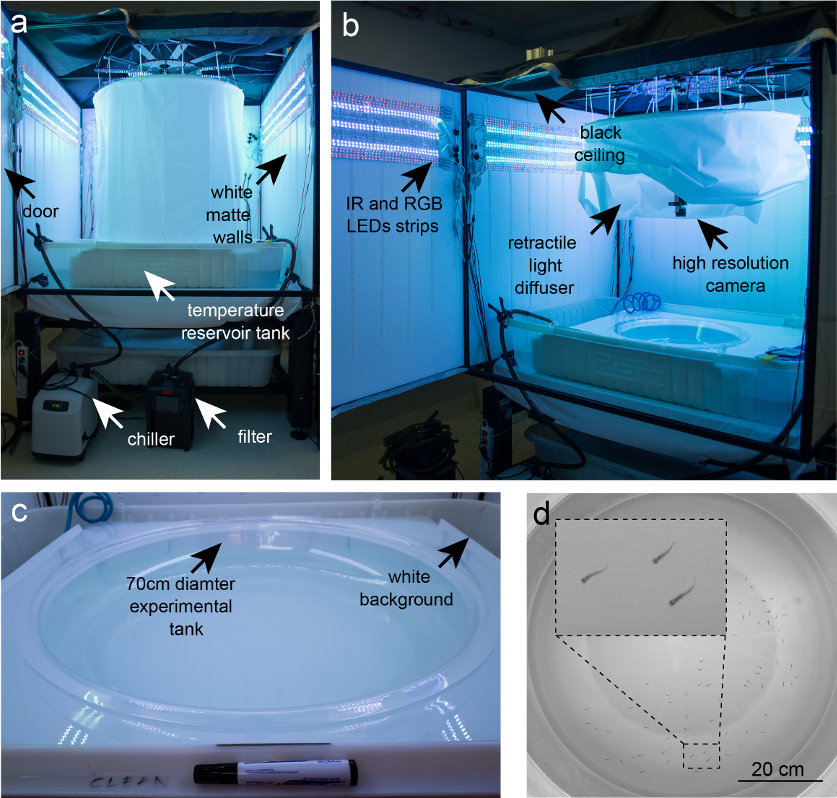
\includegraphics[width=1.0\textwidth]{figures/Experimente/Tracking/Experimentaufbau.png} 

\end{tabular}
\caption{Versuchsaufbau für die Aufnahme der Fischschwärme entnommen aus \url{https://idtrackerai.readthedocs.io/en/latest/setups.html} (besucht am 24.11.2021) \label{fig:Versuchsaufbau}  }
\end{figure}

Die Dimension des Versuchaufbaus und die Auflösung der Kamera ermöglicht das Umrechnen der Pixel in Zentimeter.
Durch die Bildrate und die Umrechnung der Pixel ist es möglich, die zurückgelegte Distanz pro Zeiteinheit zu bestimmen.
Diese Tatsache wird im weiteren Verlauf genutzt, um einen Bezug zu realen Größen zu erhalten.

\subsection{Eigene Trackingmethode}

Für das Schätzen der Bewegung von Individuen wird der optische Fluss von Farnebäck verwendet. Die Idee ist es, Individuen zwischen zwei Frames auszumachen und diese anschließend einander zuzuordnen. Hierzu wird per optischen Fluss das Bewegungsfeld zwischen zwei Frames geschätzt. Daraufhin kann ein Individuum aus dem ersten Frame zum Zeitpunkt $t$ durch das Bewegungsfeld an seine Position zum nächsten Zeitpunkt bewegt werden. Die hieraus resultierende Position sollte nahe an der realen Position des Individuums zum Zeitpunkt $t+1$ sein. Es wird also das nächstgelegene Individuum zugewiesen. Um keine doppelte Belegung zu erzeugen, steht dieses Individuum daraufhin nicht mehr zur Auswahl.

Um zu untersuchen, wie gut diese Methode funktioniert, wird anhand einer Simulation das Tracken von künstlich erzeugten Daten durchgeführt. Von Interesse ist insbesondere die Genauigkeit des Trackens in Bezug auf die Distanz, die die Agenten zurücklegen. Erwartet wird, dass ab einer bestimmten Distanz, die die Agenten pro Zeiteinheit zurücklegen, die Genauigkeit des Trackens abnimmt. Zudem ist von Interesse, welche Anzahl von Agenten diese Methode bewältigen kann.

Es sind zwei Szenarien vorgesehen, die hier betrachtet werden. In Szenario eins bewegen sich Agenten horizontal über eine Szene. Dies entspricht dem polarisierten Zustand der Fische, welcher in den Aufnahmen der realen Daten zu sehen ist. Das zweite Szenario stellt den rotierenden Zustand dar. Hierbei kreisen die Agenten um einen Mittelpunkt.


\begin{figure}[H]
\centering
\begin{tabular}{cc}
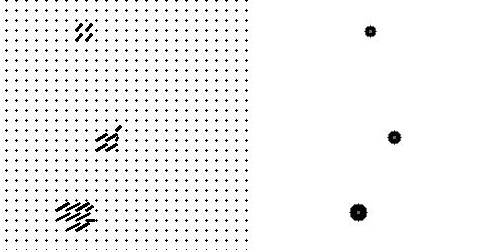
\includegraphics[width=0.5\textwidth]{figures/Experimente/Tracking/Tracking Studie.jpeg} & 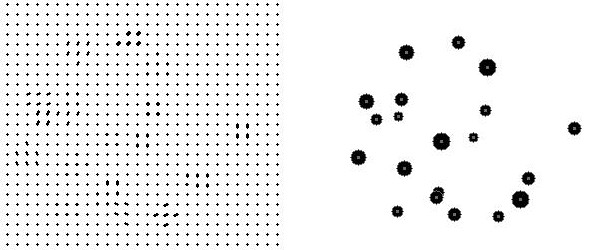
\includegraphics[width=0.5\textwidth]{figures/Experimente/Tracking/Tracking Studie Milling.jpeg}

\end{tabular}
\caption{Tracking anhand einer Simulation, horizontaler Verlauf links, rotierender Verlauf rechts\label{fig:TrackingEigen}  }
\end{figure}

Der linke Teil der jeweiligen Abbildung stellt den optischen Fluss dar. Wie zu sehen ist, verläuft die Richtung nicht exakt horizontal. Die Richtungsvektoren, welche die Agenten bewegt, wird in X- und Y-Richtung per Normalverteilung ($X \sim \mathcal{N}(0,1) $) abgelenkt. Somit bewegen sich alle Agenten etwas unterschiedlicher, im Mittelwert jedoch mit gleichbleibender Geschwindigkeit. Für die Simulation sind die Positionen der Agenten zu jeder Zeit bekannt. Das bedeutet insbesondere, dass Agenten, die sich berühren, nicht zu einer Position zusammengefasst werden, wie es der Fall ist, wenn die Positionen aus den Aufnahmen geschätzt werden müssen. Hierbei stellen Individuen, die sich berühren, ein gesondertes Problem dar, welches in diesem Versuch vernachlässigt wird.

Das Experiment wird für 10,30 und 60 Fische durchgeführt, wobei die Anzahl der Simulationsschritte 300 beträgt.


\begin{figure}[H]
\centering
\begin{tabular}{cc}
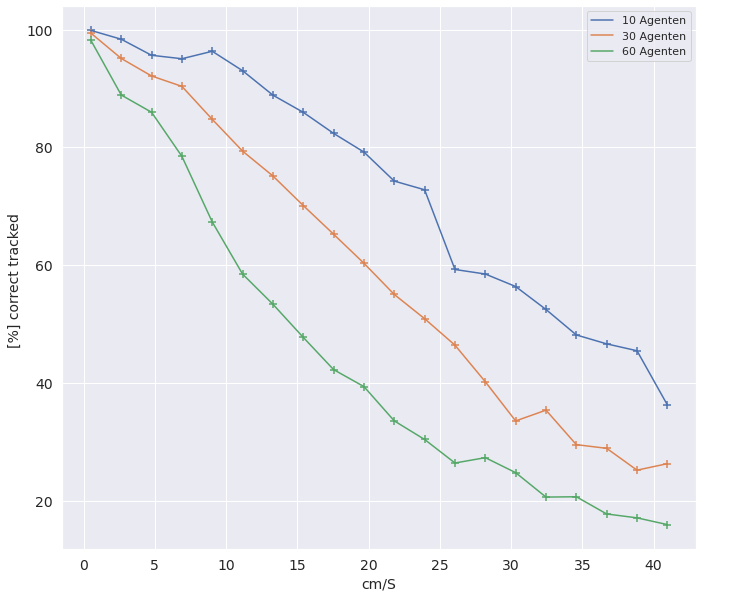
\includegraphics[width=0.7\textwidth]{figures/Experimente/Tracking/Testcaste_pol.png} 

\end{tabular}
\caption{Ergebnisse der Trackingmethode, polarisierte Bewegung\label{fig:TrackingStudyPOL}  }
\end{figure}
Das Diagramm in Abbildung \ref{fig:TrackingStudyPOL} zeigt das Resultat dieses Experimentes.
Die x-Achse beschreibt die zurückgelegte Distanz pro Sekunde. Die y-Achse die korrekte Rate der Zuweisung der Agenten.
Für die polarisierte Bewegung ist zu erkennen, dass die Anzahl der Agenten eine signifikante Rolle für die Genauigkeit des Trackens spielt. Für 10 Fische befindet sich die Genauigkeit bei $6 cm/S$ noch bei über 95\%, bei 60 Fischen hingegen bei unter 80 \%. Ebenfalls ist zu sehen, dass die Genauigkeit mit steigender Geschwindigkeit abnimmt.

\begin{figure}[H]
\centering
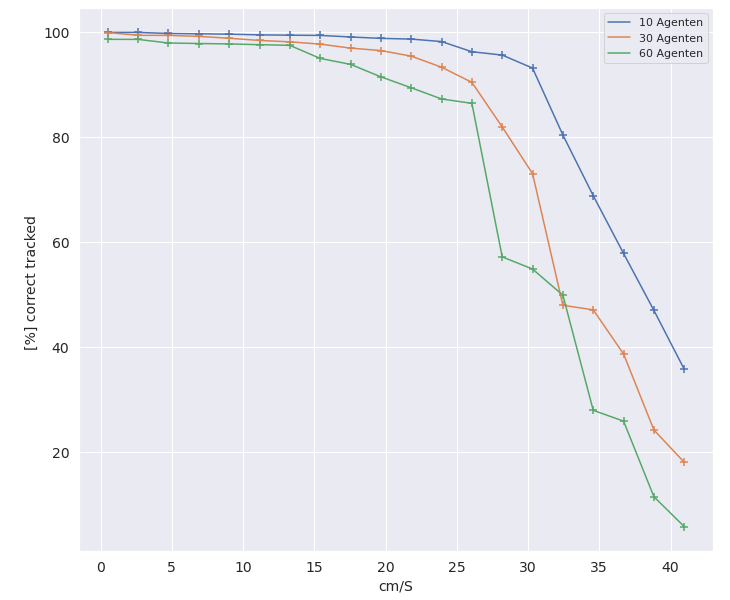
\includegraphics[width=0.7\textwidth]{figures/Experimente/Tracking/Testcaste_mil.png} 
\caption{Ergebnisse der Trackingmethode, rotierende Bewegung\label{fig:TrackingStudyMIL}  }
\end{figure}

Für die Millingformation funktioniert das Tracken wesentlich besser als für die polarisierte Formation.
Hier beginnt der Abfall der Genauigkeit erst ab ca 25 $cm/S$. Dies kann durch die bessere Verteilung der Agenten in den einzelnen Szenen erklärt werden. Während die Agenten in der polarisierten vorm hauptsächlich in direkter Nähe zueinander positioniert sind, befinden sich die Agenten in der Millingposition auf einer größeren Fläche. Hierdurch sind die Agenten nicht so nahe beieinander positioniert. Daraus resultiert eine bessere Zuordnungsrate.

Um nun zu ergründen, wie gut diese Methode auf den Realdaten funktioniert, wird mit optischem Fluss die Bewegungsvektoren der Fische zwischen einigen Paaren an Frames berechnet. Die Länge der Vektoren ergibt hierbei in etwa die zurückgelegte Strecke der Fische pro Zeiteinheit. Im Mittelwert schwimmen die Schwärme für 10 Fische ca $4 cm/S$. Die maximale Geschwindigkeit überschreitet $10 cm/S$ nicht, wodurch sich eine Genauigkeit beim Tracking von über 95\% ergibt. Für 60 Fische ergibt sich eine mittlere Geschwindigkeit von $5 cm/S$ und eine maximale Geschwindigkeit von über $8 cm/S$. Das bedeutet, dass die Genauigkeit im Mittelwert bei knapp unter $90\%$ liegt und für den maximalen Wert bei ca. $70\%$.
Für eine geringe Anzahl an Fischen scheint diese Methode ausreichend gut zu funktionieren. Will man nun Parameter approximieren, so ist es essenziell, dass die Positionen und Trajektorien der Fische so genau wie möglich sind.
Jeder Fehler mindert hierbei die Verlässlichkeit der Approximation.


\subsection{Tracking via Neural Network}
Die Trackingmethode die von \citet{DBLP:journals/corr/abs-1803-04351} verwendet wird, setzt auf künstliche neuronale Netzwerke. Die Nachfolgende Abbildung fasst die Tracking Schritte zusammen.

\begin{figure}[H]
\centering
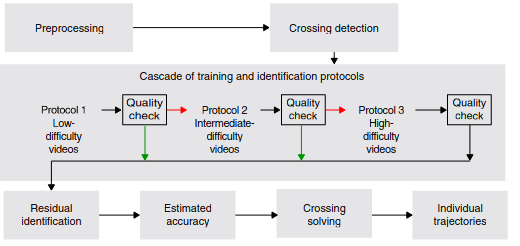
\includegraphics[width=100mm]{figures/Experimente/Tracking/AblaufTrackinb.png} 
\caption{ Ablaufdiagramm des Trackingprozesses, entnommen aus \citet{DBLP:journals/corr/abs-1803-04351}\label{fig:Ablaufdiagramm}}
\end{figure}

In einem Vorverarbeitungsschritt werden alle Individuen pro Bild extrahiert. Hierbei wird das Bild in Binärformat gebracht. Der Hintergrund wird auf null gesetzt, der Vordergrund (die Fische) auf eins.
Um herauszubekommen, welche Pixel als Hintergrund betrachtet werden, wird der Mittelwert von einigen Bildern der betrachteten Aufnahme berechnet. Subtrahiert man nun diesen Mittelwert von einem Bild der Aufnahme, so negiert sich der Hintergrund, während sich der Vordergrund abhebt (dies funktioniert nur, wenn der Hintergrund statisch ist).
Nun wird sequenzielles Labeling verwendet, um die Positionen der Fische zu berechnen. Zu kleine Regionen, welche beim Labeling extrahiert werden, werden verworfen.

Eines der Hauptprobleme des Trackings ist es, sich berührende und schneidende Individuen zu erkennen.
Dieser Schritt wird von einem künstlichen neuronalen Netzwerk übernommen.

\begin{figure}[H]
\centering
\begin{tabular}{l}
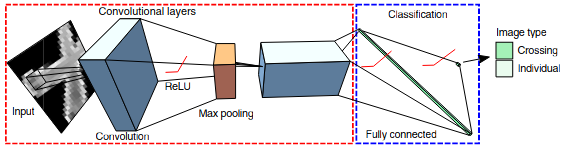
\includegraphics[width=100mm]{figures/Forschung/Individueen.png} 
\end{tabular}
\caption{ Netzwerkarchitekturen zur Klassifikation von sich berührenden und seperaten Individuen  \label{fig:tracking} entnommen aus \citet{DBLP:journals/corr/abs-1803-04351}}
\end{figure}

Die zuvor extrahierten Blobs werden durch das Netzwerk in sich schneidend und individuell klassifiziert.
Das Netzwerk wird automatisch anhand des Videos trainiert. Dazu muss die Anzahl der Individuen im Vorfeld bekannt sein. Das Datenset für das Training wird folgendermaßen zusammengestellt.Wurden exakt so viele Individuen aus dem Bild extrahiert wie vorgegeben, so werden diese extrahierten Fische als Individuen angesehen. Anderenfalls werden die extrahierten Blobs (Zusammenschluss von Pixeln) nach einem Entscheidungskriterium als sich berührend markiert. Das Kriterium ist die Abweichung der Anzahl an Pixel pro Blob. Ist diese mehr als vier Standardabweichungen vom Median entfernt, so berühren sich die Fische.
Es ist hervorzuheben, dass die Identifikation von sich berührenden Fischen auch ohne künstliches neuronales Netzwerk funktioniert. Der Laufzeitvorteil eines KNNs und die erreichbare Genauigkeit sind hierbei allerdings von Vorteil.

Daraufhin übernehmen die Protokolle 1-3 (siehe Abbildung \ref{fig:Ablaufdiagramm}) die Aufgabe das Identifikationsnetzwerk, welches in der nachfolgenden Abbildung zu sehen ist, zu trainieren.

\begin{figure}[H]
\centering
\begin{tabular}{l}
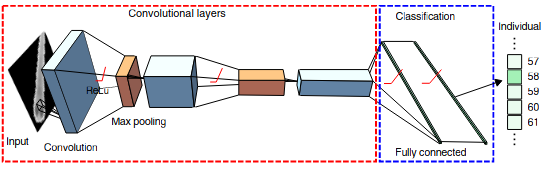
\includegraphics[width=100mm]{figures/Forschung/Identifikation.png} 
\end{tabular}
\caption{ Netzwerkarchitekturen zur ) \label{fig:Identifikation} entnommen aus \citet{DBLP:journals/corr/abs-1803-04351}}
\end{figure}

Innerhalb Protokoll 1 werden alle Intervalle zusammengestellt (pro Fisch), in denen die Fische separat voneinander sind. Diese Sequenzen sind unterschiedlich lang, enthalten aber keine Bilder von sich berührenden Fischen. Diese Intervalle werden als ''global fragment'' bezeichnet. Daraufhin wird die kürzeste Distanz ermittelt, die ein Individuum innerhalb eines ''global fragments'' zurücklegt. Diese Fragmente werden nun verwendet, um das Identifikationsnetzwerk, das in Abbildung \ref{fig:Identifikation} zu sehen ist zu trainieren. Die Protokolle 2 und 3 treten in Kraft, wenn Protokoll 1 eine unzureichende Genauigkeit im zuweisen von Identitäten aufweist.
Diese Protokolle verfeinern das Training aus Protokoll 1 um bessere Ergebnisse zu erzielen.

Das Post-processing beginnt mit dem Zuweisen der Identitäten in Form von Nummerierung (Residual identification). Hierzu wird das finale Netzwerk aus den vorherigen Trainingsschritten verwendet. Daraufhin folgt die Bestimmung der Genauigkeit mittels Bayesian Framework. Dazu werden die innerhalb der Protokolle extrahierten globalen Fragmente verwendet. Schlussendlich werden die Individuen, welche sich berühren, via Erosion und Interpolation getrennt. Aus diesen Schritten können die Trajektorien der Fische zusammengesetzt werden.

\begin{figure}[H]
\centering
\begin{tabular}{l}
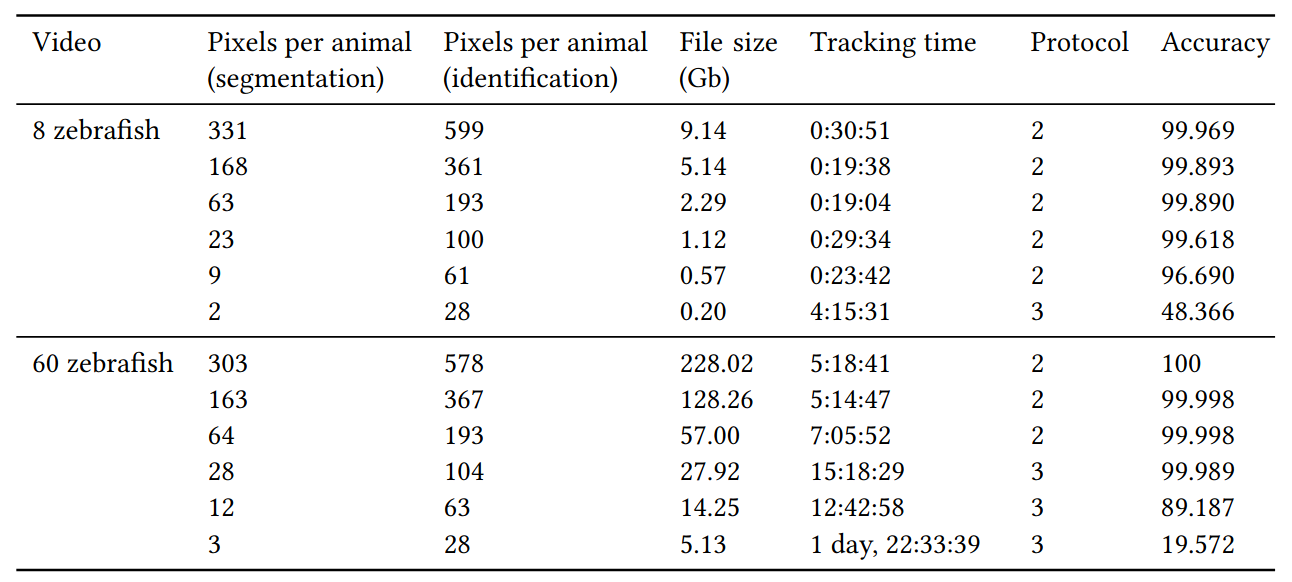
\includegraphics[width=100mm]{figures/Experimente/Tracking/resultatNN.png} 
\end{tabular}
\caption{ Auswertung der Trackinggenauigkeit \label{fig:resultatNN} entnommen aus \citet{DBLP:journals/corr/abs-1803-04351}}
\end{figure}

In Abbildung \ref{fig:resultatNN} ist die Auswertung der Trajektorien zu sehen. Hier wurden Videos von 8 und 60 Zebrafischen betrachtet. Das Tracken wurde jeweils mit unterschiedlichen Auflösungen durchgeführt.
In der Protokollspalte ist zu sehen, dass für das Training mindestens Protokoll zwei zum Einsatz kam.
Die Accuracy wurde hier von Hand durch das Inspizieren der Trajektorien anhand von 3000 Bildern durchgeführt.
Zu sehen ist, dass die Genauigkeit bei nahezu 100\% liegt. Die Trajektorien aus dieser Trackingmethode ist somit der eigenen Methode vorzuziehen und wird daher für das Approximieren der Parameter im Laufe der Thesis verwendet.
Die Trajektorien für 10,60,80 und 100 Fische stehen auf der Homepage von idtracker.ai zur Verfügung.

\subsection{Eigenschaften des Datensatzes}\label{ab:EDD}

Durch die im vorherigen Abschnitt besprochene Trackingmethode stehen die Trajektorien in Form von x-,y-Positionen pro Individuum zur Verfügung. Das ermöglicht Einsicht in das Verhalten der Schwärme.
Im vorherigen Abschnitt wurde die Geschwindigkeit der Fische mit optischem Fluss geschätzt. Nun kann durch die Positionen die exakte Geschwindigkeit pro Fisch durch die zurückgelegte Distanz zwischen zwei Frames ermittelt werden.

\begin{figure}[H]
\centering
\begin{tabular}{l}
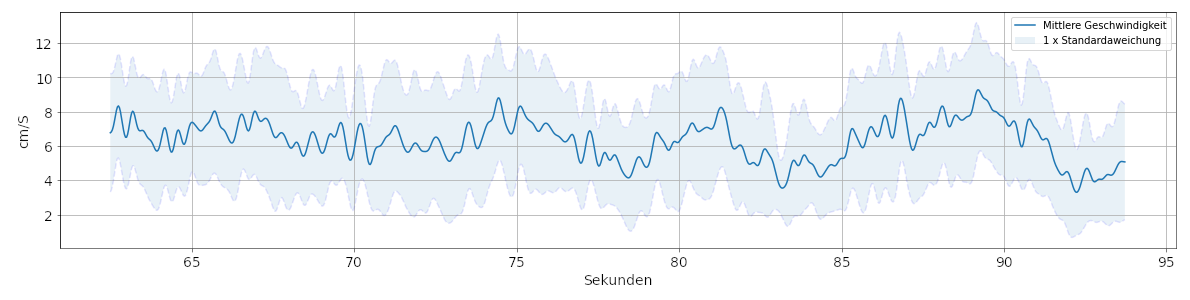
\includegraphics[width=1.0\textwidth]{figures/Experimente/Tracking/geschw_10F.png} 
\end{tabular}
\caption{ Mittlere Geschwindigkeit des Fischschwarms der Größe 10} \label{fig:geschw_10}
\end{figure}

Wie anhand der Abbildung \ref{fig:geschw_10} zu sehen ist schwankt die mittlere Geschwindigkeit des Schwarms pro Zeitschritt um 7 $cm/S$. Die geschätzte Geschwindigkeit via optischem Fluss, liegt bei $4 cm/S$. Das bedeutet, dass die tatsächliche Genauigkeit mittels eigener Trackingmethode deutlich schlechter wäre als ursprünglich angenommen.

\begin{figure}[H]
\centering
\begin{tabular}{l}
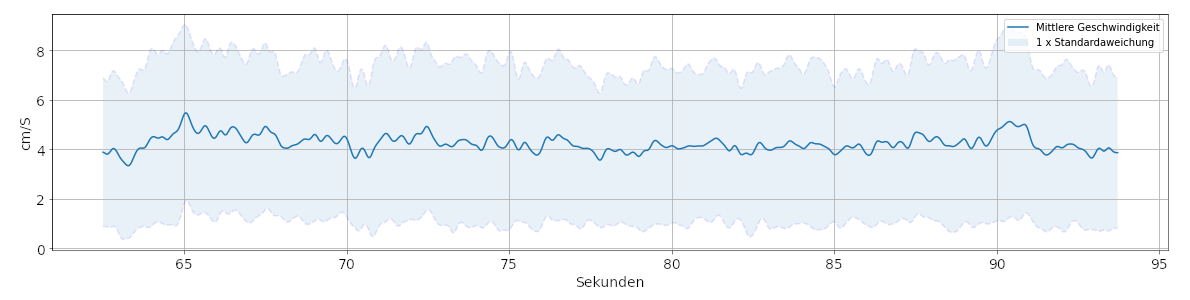
\includegraphics[width=1.0\textwidth]{figures/Experimente/Tracking/geschw_60F.png} 
\end{tabular}
\caption{ Mittlere Geschwindigkeit des Fischschwarms der Größe 60} \label{fig:geschw_60}
\end{figure}

Die mittlere Geschwindigkeit für 60 Fische liegt nahe an der mit optischem Fluss geschätzten Geschwindigkeit von $5 cm/S$. Im direkten Vergleich der beiden Diagramme kann festgestellt werden, dass die Geschwindigkeit des Schwarms mit Zunahme der Größe abnimmt. Dies kann natürlich auch dem Umstand geschuldet sein, dass sich der Schwarm in einem begrenzten Behälter befindet und ein kleinerer Schwarm mehr Raum ausnutzen kann. Dadurch kann ein Fisch eine längere Strecke geradeaus schwimmen und somit eine höhere Geschwindigkeit erreichen. Interessanterweise zeigt ein Blick auf die Geschwindigkeit des Schwarms mit 100 Individuen, dass dieser sich etwas schneller bewegt als der Schwarm mit 60 Fischen.

\begin{figure}[H]
\centering
\begin{tabular}{l}
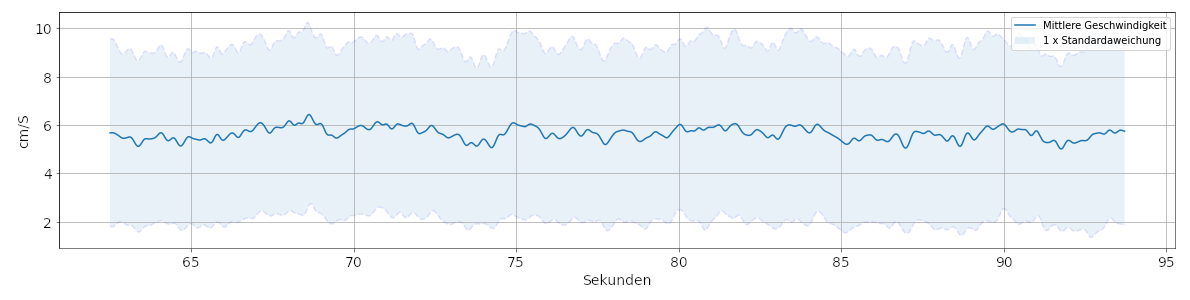
\includegraphics[width=1.0\textwidth]{figures/Experimente/Tracking/geschw_100F.png} 
\end{tabular}
\caption{ Mittlere Geschwindigkeit des Fischschwarms der Größe 100} \label{fig:geschw_100}
\end{figure}

Wie in Abbildung \ref{fig:geschw_100} zu sehen ist, liegt die mittlere Geschwindigkeit bei ca $6cm/S$.
Bei dem etwas kleineren Schwarm mit 60 Fischen hingegen bei $4cm/S$. 
Die Schwarmgröße alleine scheint die Geschwindigkeitsunterschiede nicht zu erklären.
Visualisiert man den Schwarmzustand (vgl. Abschnitt \ref{sec:Zustaende}), so kann man unterschiedliche Verhaltensweisen in Bezug auf die Schwarmgröße erkennen.

\begin{figure}[H]
\centering
\begin{tabular}{l}
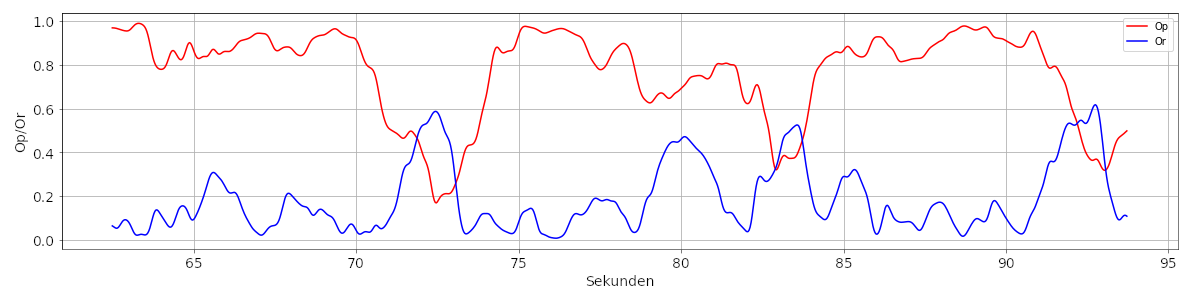
\includegraphics[width=1.0\textwidth]{figures/Experimente/Tracking/zustaende_10F.png} 
\end{tabular}
\caption{ Zustände des Fischschwarms der Größe 10} \label{fig:zust_10}
\end{figure}

\begin{figure}[H]
\centering
\begin{tabular}{l}
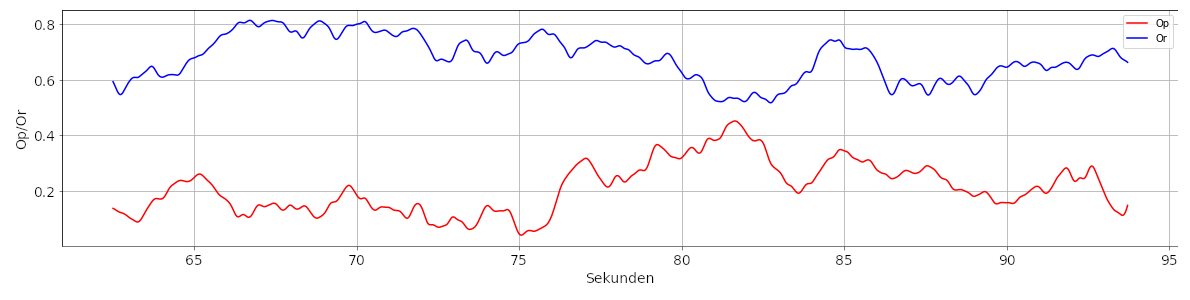
\includegraphics[width=1.0\textwidth]{figures/Experimente/Tracking/zustaende_60F.png} 
\end{tabular}
\caption{ Zustände des Fischschwarms der Größe 60} \label{fig:zust_60}
\end{figure}

\begin{figure}[H]
\centering
\begin{tabular}{l}
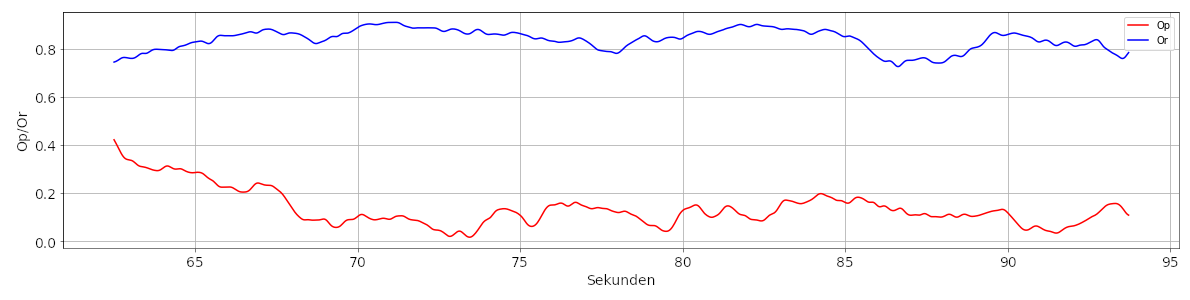
\includegraphics[width=1.0\textwidth]{figures/Experimente/Tracking/zustaende_100F.png} 
\end{tabular}
\caption{ Zustände des Fischschwarms der Größe 100} \label{fig:zust_100}
\end{figure}

In den Abbildungen \ref{fig:zust_10} - \ref{fig:zust_100} sind die Zustände Polarisation und rotierend zu sehen. Blau ist hier der Rotationszustand und rot der polarisierte Zustand. Es ist deutlich zu erkennen, dass bei dem kleineren Schwarm mit 10 Fischen der polarisierte Zustand dominiert. Je größer der Schwarm ist, desto stärker geht er in den Rotationszustand über. Nun sieht man, dass beim Schwarm mit 60 Fischen der polarisierte Zustand noch teilweise vorhanden ist. Beim Schwarm mit 100 Fischen dominiert hingegen der Rotationszustand. Dies könnte den Geschwindigkeitsunterschied zwischen 100 und 60 Fischen, der zuvor ausgemacht wurde, erklären. Die Beobachtung ist somit, dass Schwärme, die sich in einem eindeutigen Zustand befinden, eine höhere Bewegungsgeschwindigkeit aufweisen als Schwärme, deren Zustände weniger klar definiert sind.

\section{Approximation Anhand künstlich erzeugter Daten}

In diesem Teil des Kapitels werden zu Beginn die beiden Optimierungsverfahren verglichen.
Hierbei wird die Laufzeit der Algorithmen sowie die Qualität des erreichten Optimums begutachtet.
Ziel in diesem Experiment ist es, die beiden Opimierungsverfahren gegenüberzustellen und herauszufinden, welcher Algorithmus in welchen Situationen zu bevorzugen ist.

Hierzu werden durch die vorgestellten Modelle künstliche Daten generiert. Initial werden den Agenten Positionen zugewiesen, die aus einer Gleichverteilung stammen. Dadurch ist die Dichte der Agenten nicht zu hoch, wie es beispielsweise bei einer Normalverteilung der Fall wäre. Das würde zur Folge haben, dass die Agenten zu Beginn konzentriert um den Mittelwert positioniert sind und dadurch zuerst den Abstand herstellen müssten. Für das Boids Modell ist in diesem Fall nur die Abstandhaltenzone relevant.
Jeder Agent bekommt zu Beginn einen Richtungsvektor, der aus einer Gleichverteilung gezogen wird, zugewiesen. Dieser Vektor wird hierfür normiert. Dies ist nötig, um den Agenten eine Startrichtung zu geben. Wie in Abschnitt \ref{sec:Modelle} diskutiert, benötigen Agenten die sich in keiner Nachbarschaft befinden einen Richtungsvektor. Ohne diesen kann der Richtungsvektoren welcher sich aus der Orientierungszone ergibt, nicht errechnet werden.


% subsection subsection_name (end)
\subsection{Vergleich zwischen PSO und RMD}

Das Ziel dieses Vergleiches ist zu erörtern, wie die beiden Algorithmen in einem einfachen Szenario performen. Hierzu wird eine zufällige Sequenz erzeugt, die für beide Algorithmen gleich ist.

Die Algorithmen sollen nun das Parameterset bestimmen, die diese Sequenz erzeugt. Hierbei interessiert, ob die Parameter korrekt bestimmt wurden und wie lange die Algorithmen für die Bestimmung benötigen.

Es wurden 3 Szenarien mit unterschiedlicher Schwarmgröße und gleichen Parametern erstellt.
Die Schwarmgrößen sind 10,50 und 100 Agenten. Beide Algorithmen wurden 1000 Iterationen durchlaufen.
Die Lernrate für RMD ist $1e-2$ und die Anzahl der Partikel für PSO ist 50 pro Dimension.

Als Fehlerfunktion wird die $L2$ Verlustfunktion verwendet, diese ist definiert durch:


\begin{subequations}
\begin{align*}
L2Loss &= \sum_i^n(Y_{true} - Y_{pred})^2
\end{align*}
\end{subequations}

Es wird hierbei die Distanz zwischen der korrekten Agenten Position und der vorhergesagten Agenten Position bestimmt.
Durch die Quadrierung werden Distanzunterschiede stärker bestraft.

\textbf{Metrisches Boids Modell}

Das Boids Modell muss für diesen Versuch verändert werden. Das grundlegende Problem ist, dass die Parameter nicht Teil des Graphen sind (siehe Abschnitt \ref{sec:RMD}). Die Agenten werden in Folge einer binären Entscheidung den Zonen zugeordnet. Ist ein Agent innerhalb der Abstandhaltenzone, so wird er für die Berechnung mit einbezogen, anderenfalls nicht. Die Berechnung der neuen Richtung wird dadurch nur indirekt durch die Zonen bestimmt. Somit werden die Parameter nicht bis zur Fehlerfunktion durchgereicht, wodurch die Ableitung bestimmt wird.

Nun kann man auch die Distanzen der Agenten $i$ zu dem betrachteten Agenten $j$ mit dem Radius der jeweiligen Zone skalieren.
Das führt dazu, dass, falls die Agenten $i$ relevant sind, diese innerhalb des Einheitskreises um den Agent $j$ liegen. Die Agenten mit dem Abstand größer als eins, werden dementsprechend ignoriert. Das hat zur Folge, dass die Radien per Skalierung in dem Ableitungsgraphen auftauchen und nach diesen abgeleitet werden kann. Der Einschlagwinkel und der Winkel der blinden Zone werden zunächst als konstant angenommen.

\begin{figure}[h]
\centering
\begin{tabular}{cc}
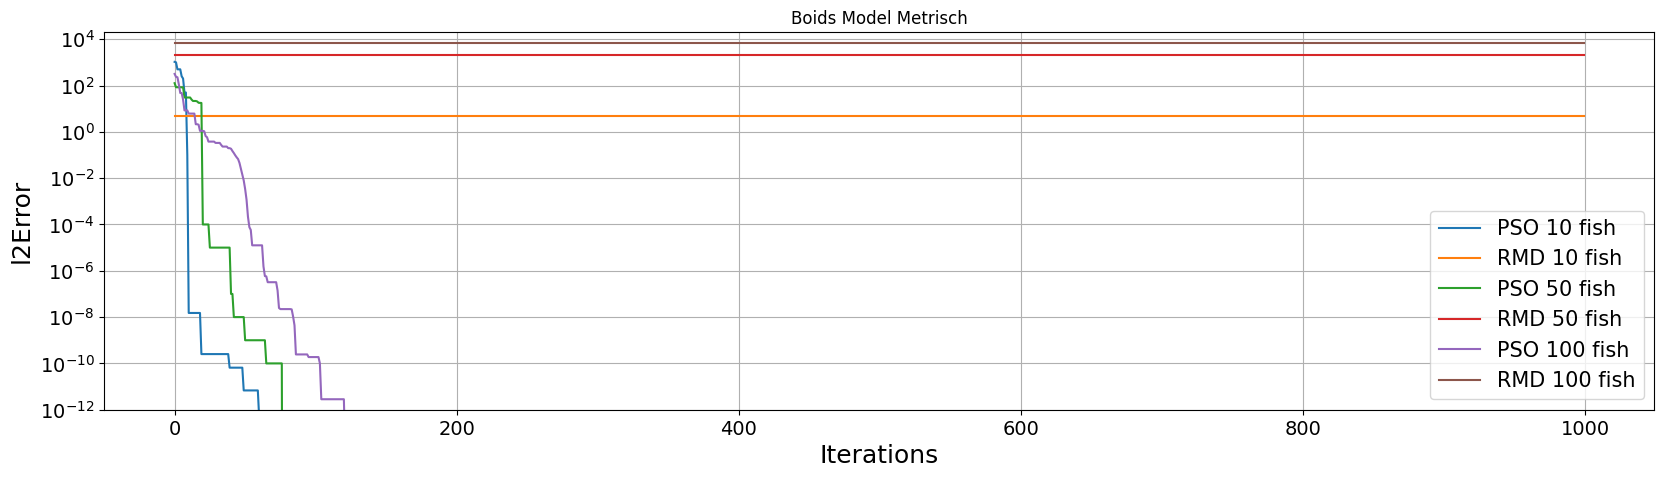
\includegraphics[width=1.0\textwidth]{figures/Experimente/Boids_Laufzeit.png} 

\end{tabular}
\caption{PSO vs. RMD anhand von Boids \label{fig:BOIDS_PSOVSRMD} }
\end{figure}

Wie anhand der Abbildung \ref{fig:BOIDS_PSOVSRMD} zu erkennen ist, erreicht der PSO Algorithmus im Falle des Boids Modells für alle Agentenanzahlen einen minimalen Fehlerwert. Hierfür wird nicht mehr als 200 Iterationen benötigt.

Bei RMD hingegen ist keine Fehlerveränderung festzustellen. Beim Betrachten der Parameter konnte festgestellt werden, dass sich keine Veränderung einstellt. Die Laufzeit ist hierbei nicht relevant, da sich der Fehler im Falle des RMD nicht verbessert.
Somit ist hier PSO zu bevorzugen.

\textbf{Eigenes Modell}

\begin{figure}[h]
\centering
\begin{tabular}{cc}
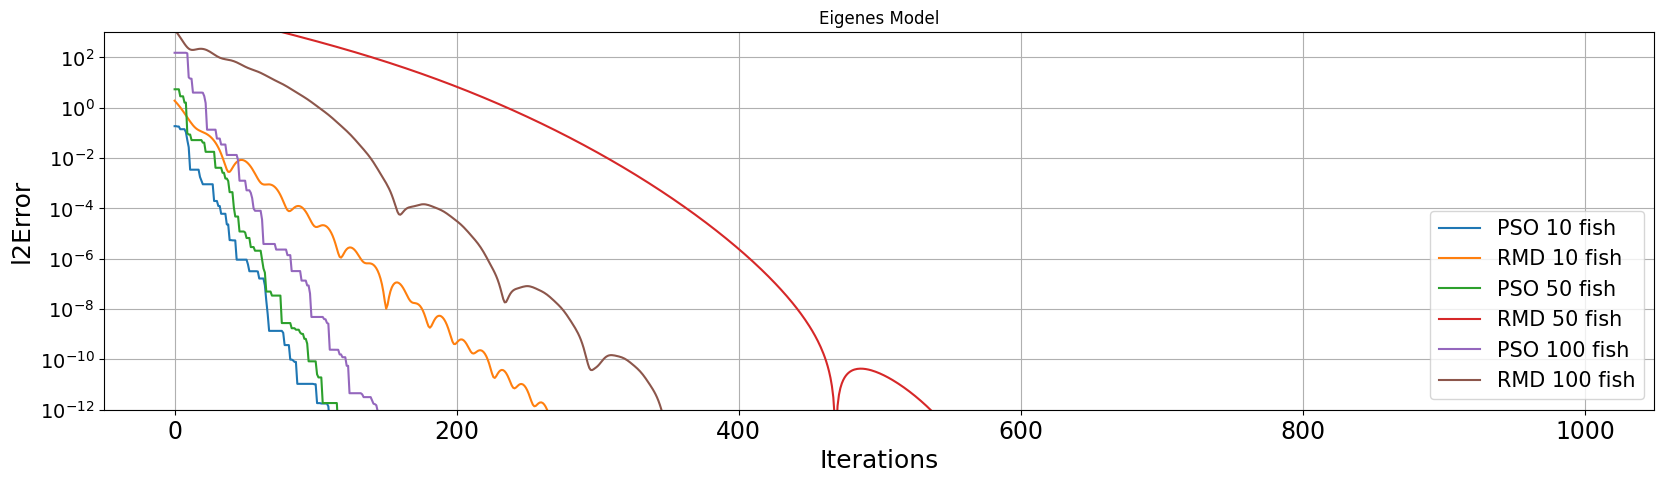
\includegraphics[width=1.0\textwidth]{figures/Experimente/Eigenes_Laufzeit.png} 
\end{tabular}
\caption{PSO vs. RMD Anhand des eigenen Modells \label{fig:Eigen_PSOVSRMD}}
\end{figure}

Abbildung \ref{fig:Eigen_PSOVSRMD} zeigt, dass sich für beide Verfahren eine Verbesserung des Fehlers einstellt.
PSO benötigt für alle Agentenanzahlen weniger Iterationen als RMD. 
Für die Laufzeitbestimmung wurden die Versuche pro Anzahl der Agenten zehnmal durchgeführt.
In folgender Tabelle ist der Mittelwert der jeweiligen Laufzeiten für 1000 Iterationen zu sehen.

\begin{table}[h]
	\centering
	\begin{tabular}{ccc}
	Anzahl Agenten & Laufzeit in Sekunden PSO & Laufzeit in Sekunden RMD \\
	\hline
	10 & 85.5 & 0.6 \\
	50 & 262 & 1.3\\
	100 & 598 & 2.6\\
	\end{tabular}
	\caption{\textit{Vergleich der Laufzeiten zwischen PSO und RMD}}
			\label{table:Laufzeiten}
\end{table}

Zu erkennen ist, dass PSO in allen Szenarien schlechtere Laufzeiten liefert. 
Auch wenn PSO weniger Iterationen benötigt als RMD ist PSO aufgrund des großen Laufzeitunterschiedes nicht verwendbar. Aus diesem Grund wird für dieses Modell im Laufe der Arbeit der RMD Algorithmus verwendet.

\subsection{Approximierung von konstanten Parametern}\label{AVKP}


Für diesen Teil der Arbeit werden künstliche Daten mit konstanten Parametern erzeugt.
Initial werden den Agenten wieder zufällige Positionen und Richtungsvektoren zugewiesen. Anhand der Daten sollen die Parameter geschätzt werden, die diese Sequenzen erzeugen.

\subsubsection{Metrisches Boids Modell}

Wie zuvor erörtert, ist für dieses Modell PSO zu verwenden. Es werden wieder 50 Partikel pro Dimension verwendet, die Anzahl der Iterationen, bis die Suche nach Parametern abgebrochen wird ist 300.


Die Simulation, auf die sich die nachfolgenden Abbildungen beziehen, sind mit 10 Agenten durchgeführt worden.
\begin{figure}[H]
\centering
\begin{tabular}{cc}
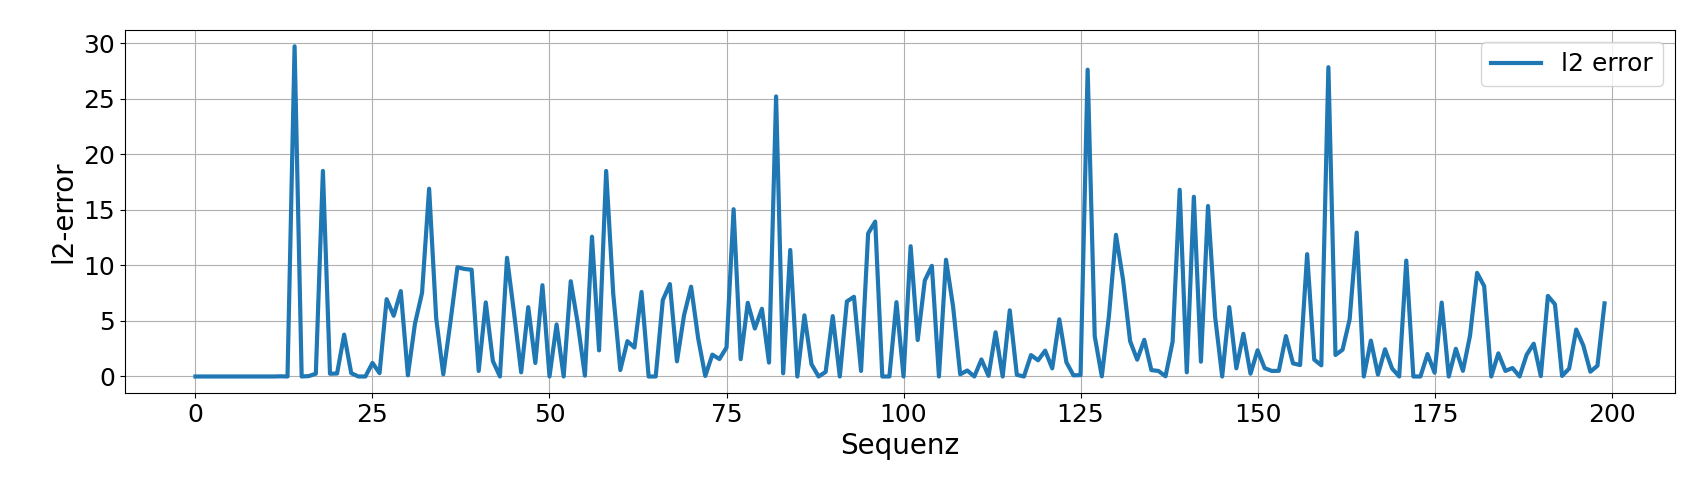
\includegraphics[width=1.0\textwidth]{figures/Experimente/10Fisch/l2error_StatischeParameter.png} 
\end{tabular}
\caption{L2-Fehler der konstanten Parametervorhersage \label{fig:l2errorBoids10FischeStatisch}}
\end{figure}

Der l2-Fehler in Abbildung \ref{fig:l2errorBoids10FischeStatisch} ist in den ersten Sequenzen nahe an null und wird daraufhin größer. In dem vorherigen Versuch, wurden nur zwei aufeinanderfolgende Sequenzen betrachtet. Hier werden hingegen mehrere aufeinanderfolgende Sequenzen betrachtet. Hier ist es nun der Fall, dass die Vorhersage zum Zeitpunkt $t$, als Input für die Vorhersage zum Zeitpunkt. $t+1$ genutzt wird. Das hat zur Folge, dass die zukünftigen Sequenzen von deren Vorgängern abhängig sind. 
Zu erkennen ist, dass der Fehler immer wieder auf null zurückspringt.

Zudem schwankt der $L2$-Fehler von Sequenz zu Sequenz sehr stark.
Eine Explosion des Fehlers in dem Sinne, dass dieser unweigerlich größer wird, ist hier nicht festzustellen.
Wie anhand der x-Achse zu sehen ist, wurden hier Parameter für 200 Sequenzen bestimmt.
Die aus der Approximation resultierenden Parameter sind in den nächsten Abbildungen zu sehen.
Hierbei ist anzumerken, dass diese mittels Gaußglocke geglättet wurden, um das Rauschen der vorhergesagten Parameter zu unterdrücken. Der Parameter $\sigma$ der Gaußglocke wurde für die Glättung auf den Wert 6 gesetzt.

\begin{figure}[H]
\centering
\begin{tabular}{cc}
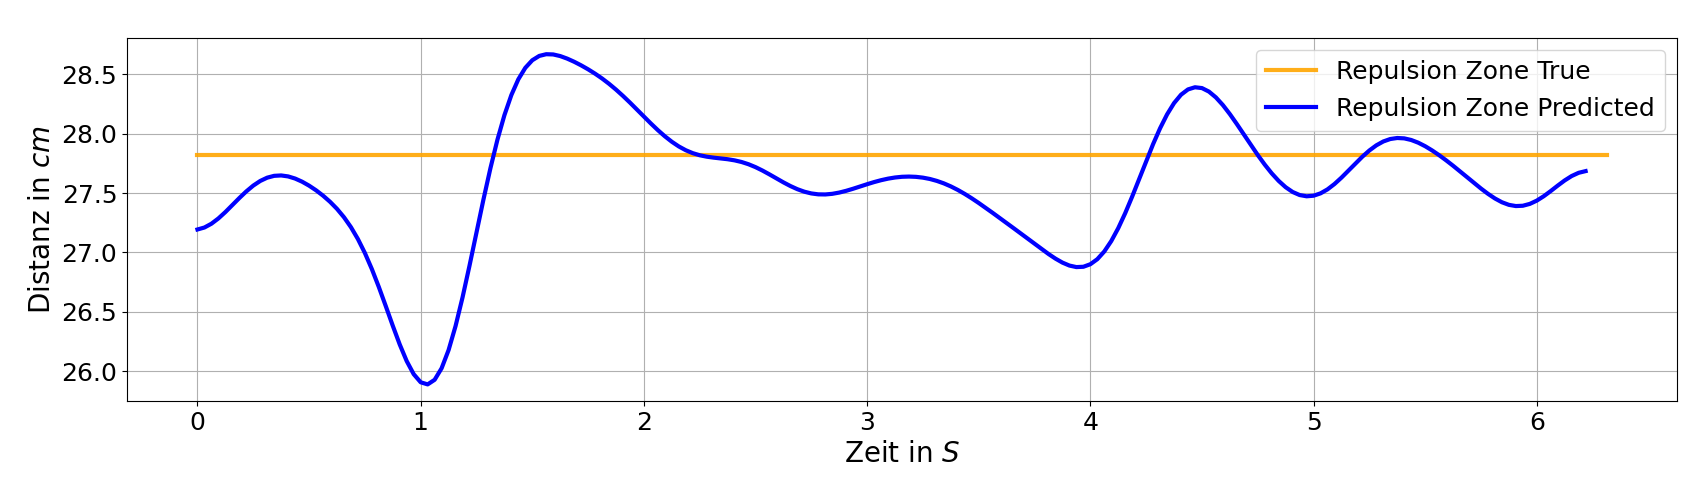
\includegraphics[width=1.0\textwidth]{figures/Experimente/10Fisch/RepulsionZone.png} 
\end{tabular}
\caption{Vorhergesagte Abstandhalten-Zonen in Blau vs korrekte Zonen in Orange  \label{fig:RZonePrediction}}
\end{figure}

\begin{figure}[H]
\centering
\begin{tabular}{cc}
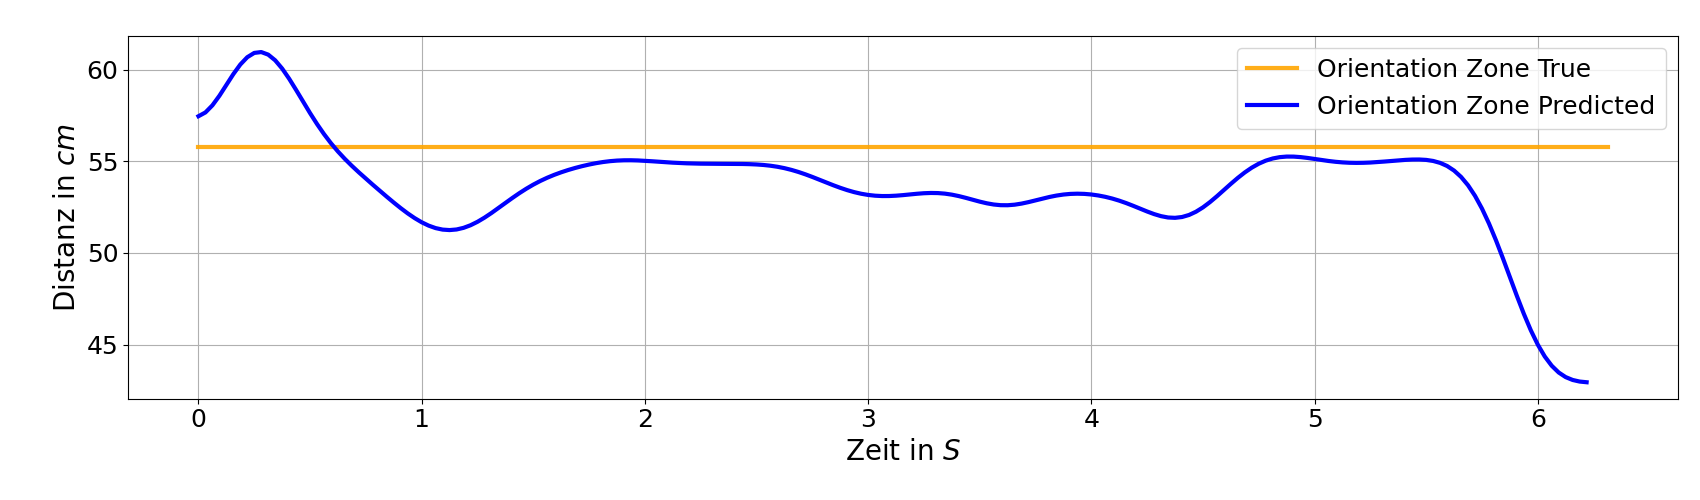
\includegraphics[width=1.0\textwidth]{figures/Experimente/10Fisch/OrientationZone.png} 
\end{tabular}
\caption{Vorhergesagte Orientierungs-Zonen in Blau vs korrekte Zonen in Orange  \label{fig:OZonePrediction}}
\end{figure}

\begin{figure}[H]
\centering
\begin{tabular}{cc}
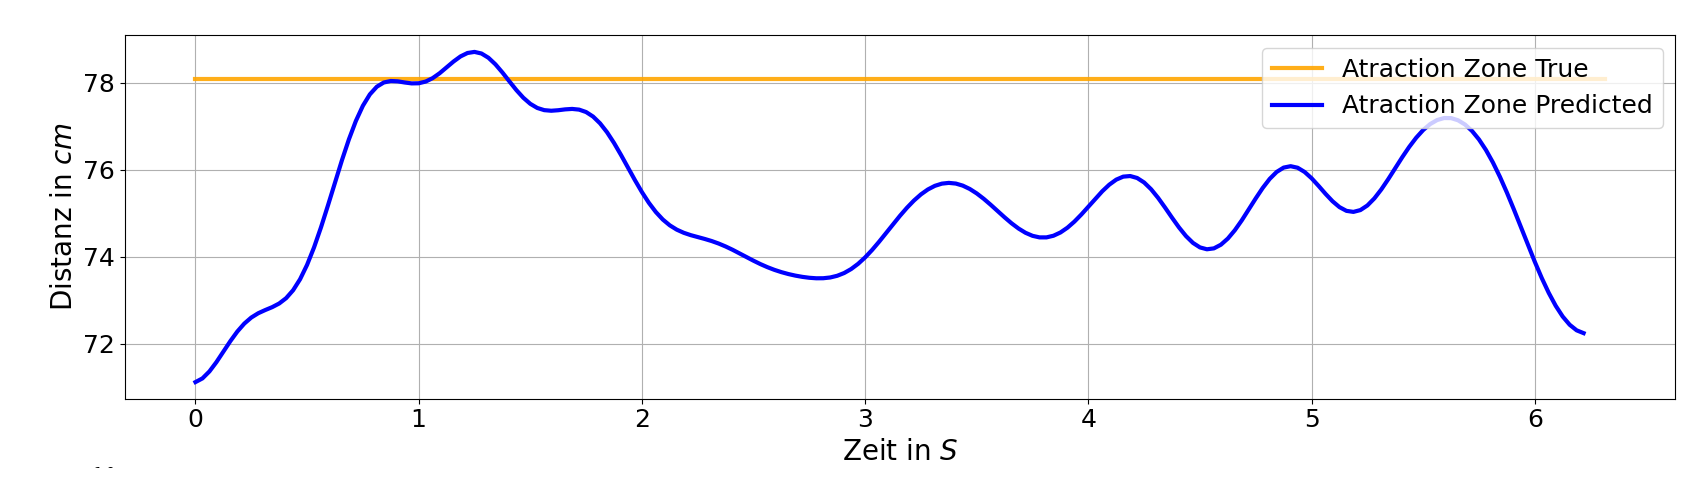
\includegraphics[width=1.0\textwidth]{figures/Experimente/10Fisch/AttractionZone.png} 
\end{tabular}
\caption{Vorhergesagte Zusammenhalten-Zonen in Blau vs korrekte Zonen in Orange  \label{fig:AZonePrediction}}
\end{figure}

Die x-Achse spiegelt die Zeit wieder und die y-Achse der Radius der jeweiligen Zone in Zentimetern. In den Abbildungen \ref{fig:RZonePrediction}-\ref{fig:AZonePrediction} sind die konstanten Simulationsparameter für die jeweiligen Zonen zu sehen. Es ist ersichtlich, dass die vorhergesagten Parameter für die Zonen nicht konstant sind.
Dies ist nicht verwunderlich, denn die Zonen des Boids Modells sind nicht sensibel gegenüber Veränderung.
Ist beispielsweise ein Agent in der Orientierungszone, dann ist es nicht relevant, wie groß die Zone ist, solange nur dieser eine Agent in der Zone vorhanden ist. Selbiges gilt für die anderen Zonen.

Die Vorhersage der Winkel $\theta$ zur Begrenzung des Einschlagwinkels und $\alpha$, welches den Winkel des blinden Kegels hinter dem Agenten steuert, ist in den nachfolgenden Abbildungen zu sehen.

\begin{figure}[H]
\centering
\begin{tabular}{cc}
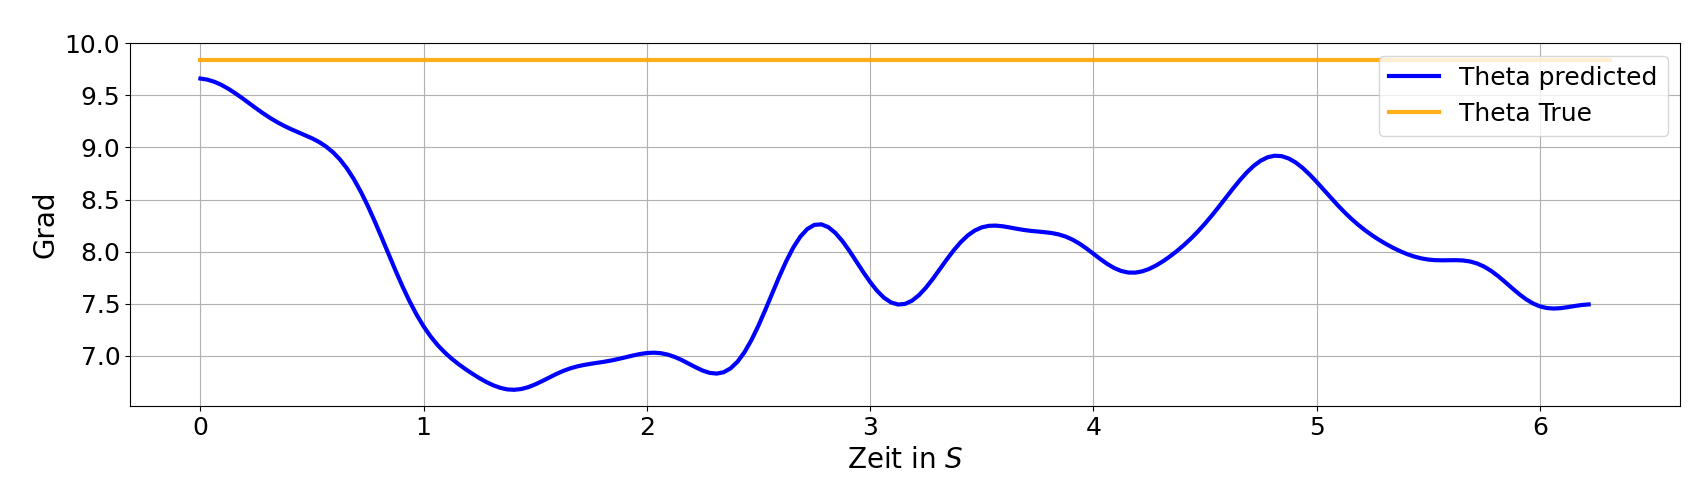
\includegraphics[width=1.0\textwidth]{figures/Experimente/10Fisch/Theta.png} 
\end{tabular}
\caption{Vorhergesagter Einschlagswinkel in Blau vs korrekter Winkel in Orange \label{fig:AlphaStatischPrediction}}
\end{figure}


Der maximale Einschlagswinkel in Abbildung \ref{fig:AlphaStatischPrediction} wird niedriger vorhergesagt, als er tatsächlich ist. Tatsächlich sollte er bei ca. 10 Grad sein, die Vorhersage liegt im Mittel etwa bei 8 Grad.


\begin{figure}[H]
\centering
\begin{tabular}{cc}
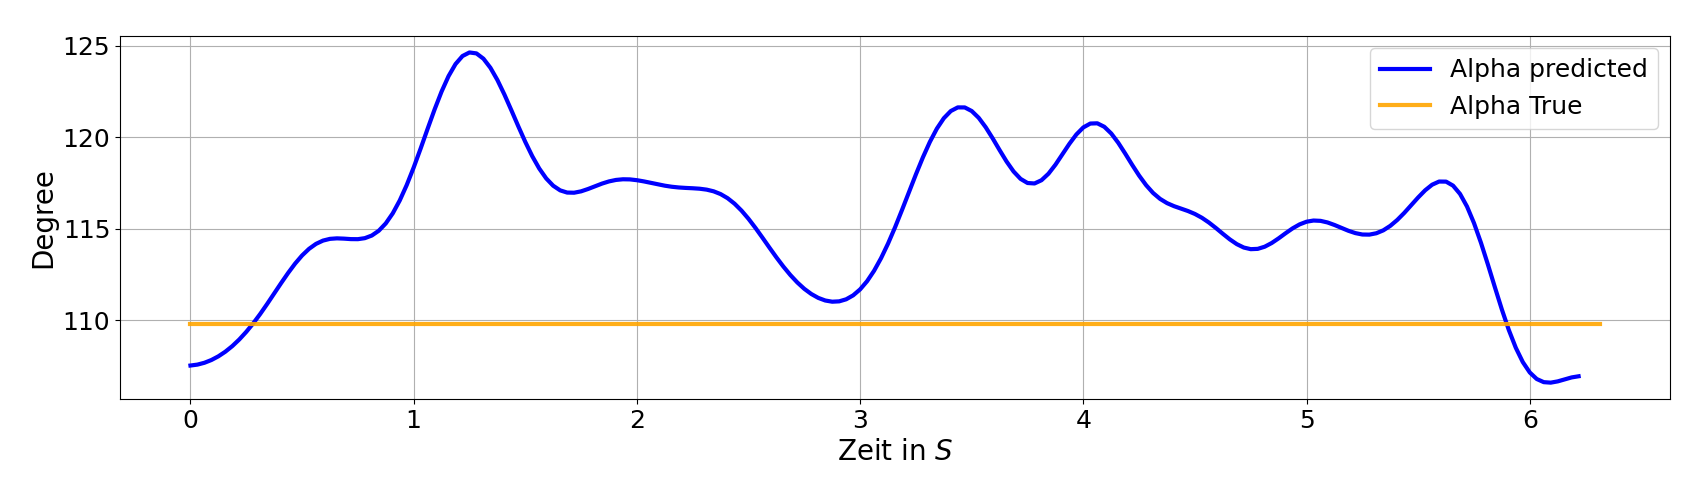
\includegraphics[width=1.0\textwidth]{figures/Experimente/10Fisch/Alpha.png} 
\end{tabular}
\caption{Vorhergesagte Winkel der blinden Zone in Blau vs korrekter Winkel in Orange \label{fig:AlphaStatischPrediction}}
\end{figure}

Der Winkel $\alpha$ der den Blindspot definiert, wird hingegen höher vorhergesagt, als er tatsächlich ist. Somit nimmt der Agent in der Vorhersage weniger Einfluss von Agenten im hinteren Bereich als Agenten, die der korrekten Simulation zugehörig sind.


Schaut man sich nun die Zustände an, so wird deutlich, dass unterschiedliche Parameter ähnliche Statusverläufe erzeugen können.
Die Diagramme wurden ebenfalls mittels Gaußglocke geglättet wobei der Parameter $\sigma = 6$ gesetzt wurde.
Die ungeglätteten Diagramme sind im Anhang zu sehen.

\begin{figure}[H]
\centering
\begin{tabular}{cc}
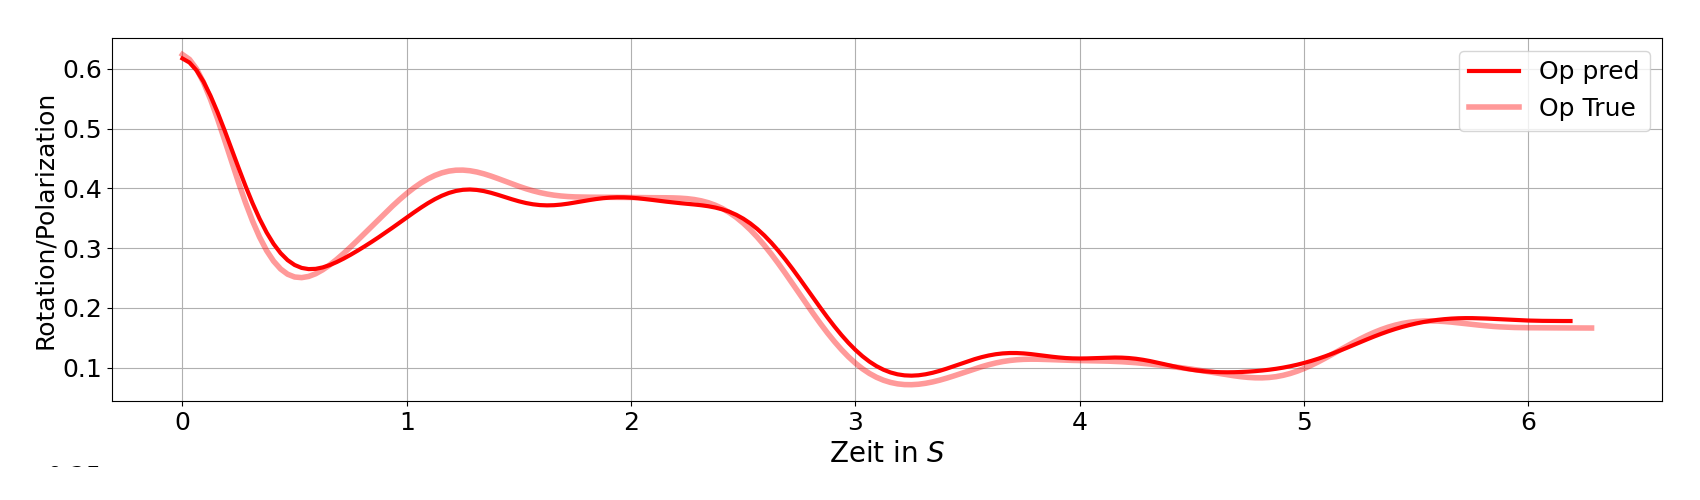
\includegraphics[width=1.0\textwidth]{figures/Experimente/10Fisch/Polarisierung.png} 
\end{tabular}
\caption{Polarisierungszustand der Simulation im Vergleich zur Vorhersage \label{fig:Pol10FischeStatisch}}
\end{figure}

In Abbildung \ref{fig:Pol10FischeStatisch} ist der Polarisationszustand der Simulation (transparent) sowie der Vorhersage (intransparent) zu sehen. Es ist zu erkennen, dass die Zustände nahe beieinander liegen, woraus sich schließen lässt, dass Vorhersage und Simulation über die Zeit hinweg ähnlich polarisiert sind. Hier ist hervorzuheben, dass wie in Abschnitt \ref{sec:Zustaende} besprochen, keine eindeutige Polarisierung vorzufinden ist. Die Kurve liegt in allen Bereichen unter 0.65.

\begin{figure}[H]
\centering
\begin{tabular}{cc}
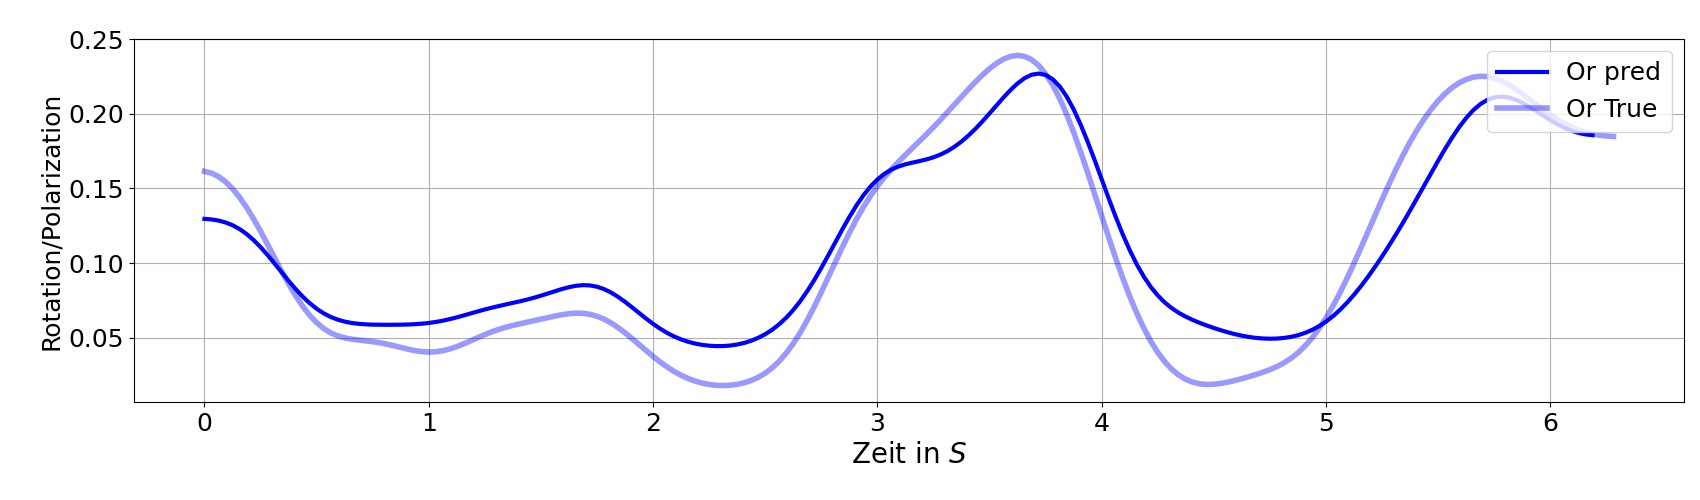
\includegraphics[width=1.0\textwidth]{figures/Experimente/10Fisch/Rotation.png} 
\end{tabular}
\caption{Rotationszustand der Simulation im Vergleich zur Vorhersage \label{fig:Rot10FischeStatisch}}
\end{figure}

Die obige Abbildung zeigt ebenfalls, dass die Zustände ähnlich verlaufen. Die Simulation und dessen Vorhersage rotieren demzufolge in ähnlicher Weiße. Auch hier muss erwähnt werden, dass kein Rotationszustand erreicht wurde, da in allen Fällen $O_r < 0.65$ ist.


\begin{figure}[H]
\centering
\begin{tabular}{cc}
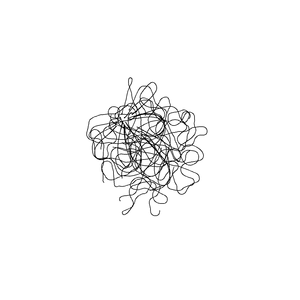
\includegraphics[width=0.5\textwidth]{figures/Experimente/10Fisch/Boids_sim_fake.png}&
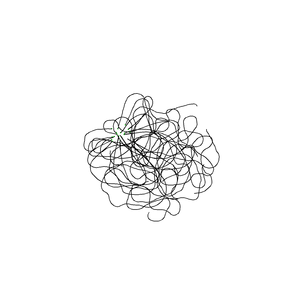
\includegraphics[width=0.5\textwidth]{figures/Experimente/10Fisch/Boids_sim_fake1.png}
\end{tabular}
\caption{Trajektorien der künstlich erzeugten Daten (links) und der mittels approximierten Parametern (rechts) \label{fig:AP}}
\end{figure}

Das Betrachten der Laufwege der künstlichen Daten und der Simulation mittels approximierten Parametern zeigt, dass unterschiedliche Laufwege das Resultat dieses Experimentes sind. Es ist zu sehen, dass sich beide Simulationen ähneln. Es existiert kein Ausreißer, welche das eine Bild vom anderen abheben lässt.



\subsubsection{Eigenes Modell}

Für das eigene Modell gelten dieselben Ausgangssituationen wie für das metrische Modell. Für die Approximation wird RMD verwendet.
Die Lernrate ist $0.02$ und zum Anpassen der Lernrate wird ADAM verwendet. Hier werden pro Approximation nicht mehr als 2000 Iterationen durchlaufen.

\begin{figure}[H]
\centering
\begin{tabular}{cc}
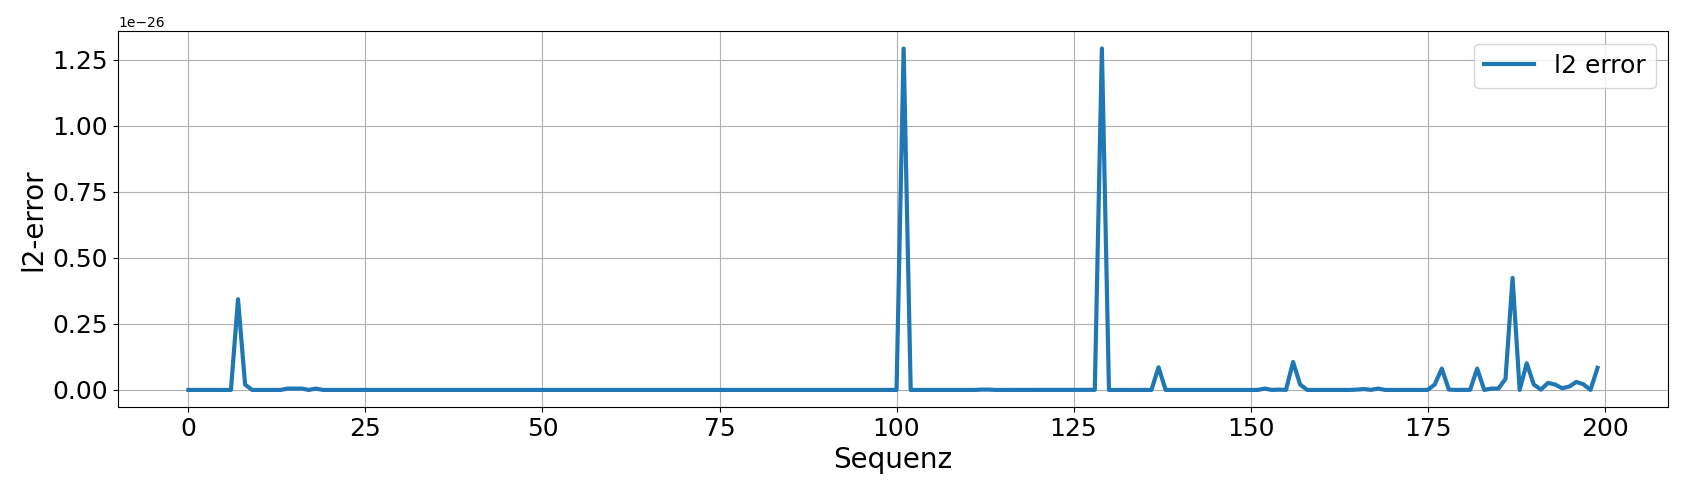
\includegraphics[width=1.0\textwidth]{figures/Experimente/10Fisch/PWD_l2error.png} 
\end{tabular}
\caption{L2 Fehler für das eigene Modell \label{fig:PWD_l2error}}
\end{figure}

In der Abbildung \ref{fig:PWD_l2error} ist der Fehler des eigenen Modells zu sehen. Der Fehler liegt ausnahmslos bei null.
Daraus kann geschlossen werden, dass die Vorhersage mit der künstlichen Simulation übereinstimmt.


\begin{figure}[H]
\centering
\begin{tabular}{cc}
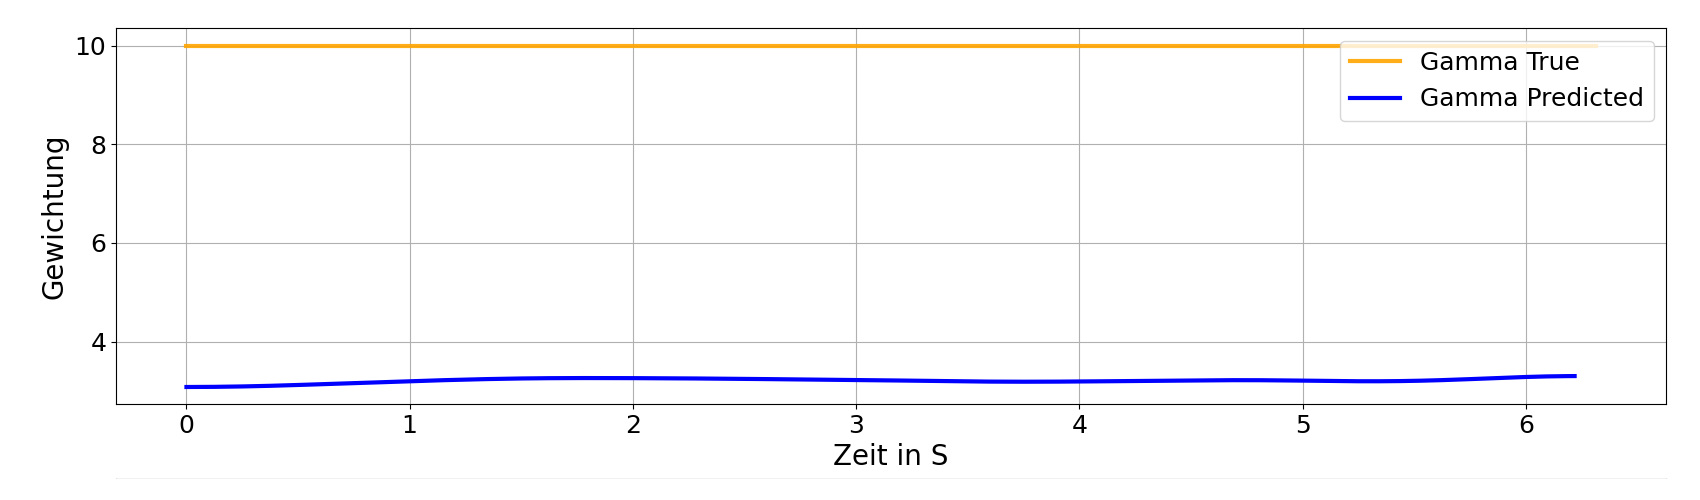
\includegraphics[width=1.0\textwidth]{figures/Experimente/10Fisch/PWD_Gamma.png} 
\end{tabular}
\caption{L2 Fehler für das eigene Modell \label{fig:PWD_Gamma}}
\end{figure}

Ein Blick auf den Parameter Gamma zeigt, dass die Vorhersage ziemlich konstant bei ca. 3 liegt und somit nicht dem korrekten Parameter von 10 entspricht.

\begin{figure}[H]
\centering
\begin{tabular}{cc}
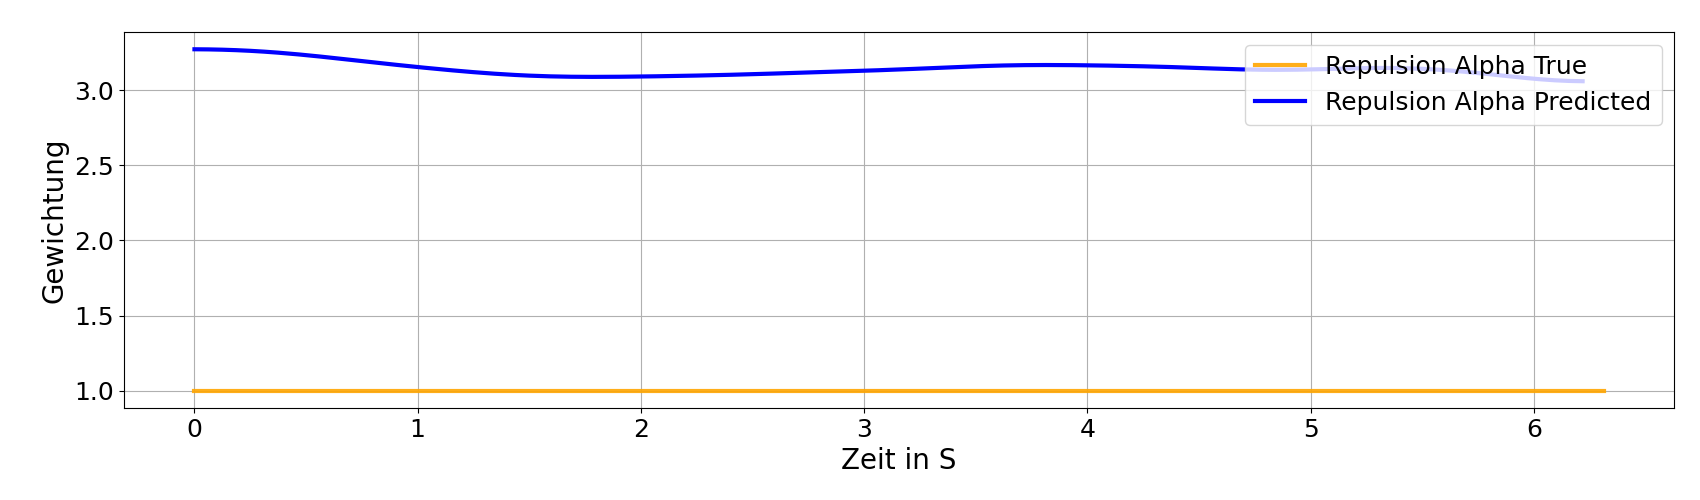
\includegraphics[width=1.0\textwidth]{figures/Experimente/10Fisch/PWD_alpha1.png} 
\end{tabular}
\caption{Parameter $\alpha_1$ für das eigene Modell \label{fig:PWD_Alpha1}}
\end{figure}

\begin{figure}[H]
\centering
\begin{tabular}{cc}
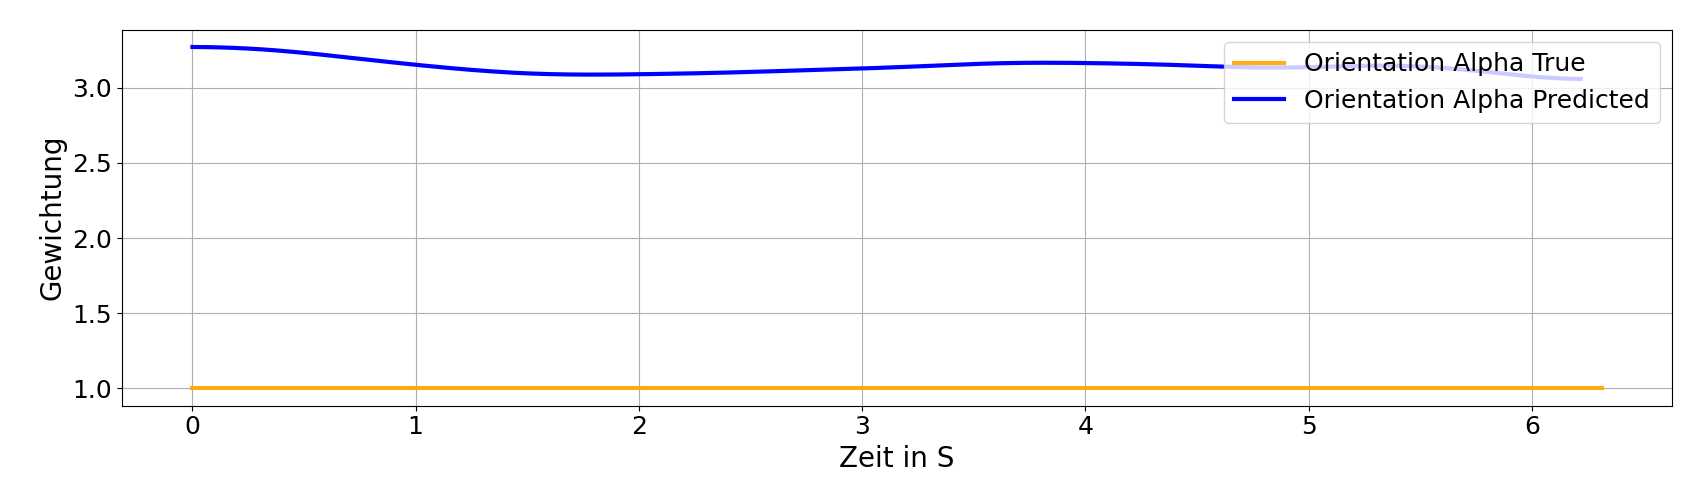
\includegraphics[width=1.0\textwidth]{figures/Experimente/10Fisch/PWD_alpha2.png} 
\end{tabular}
\caption{Parameter $\alpha_2$ für das eigene Modell \label{fig:PWD_Alpha2}}
\end{figure}



\begin{figure}[H]
\centering
\begin{tabular}{cc}
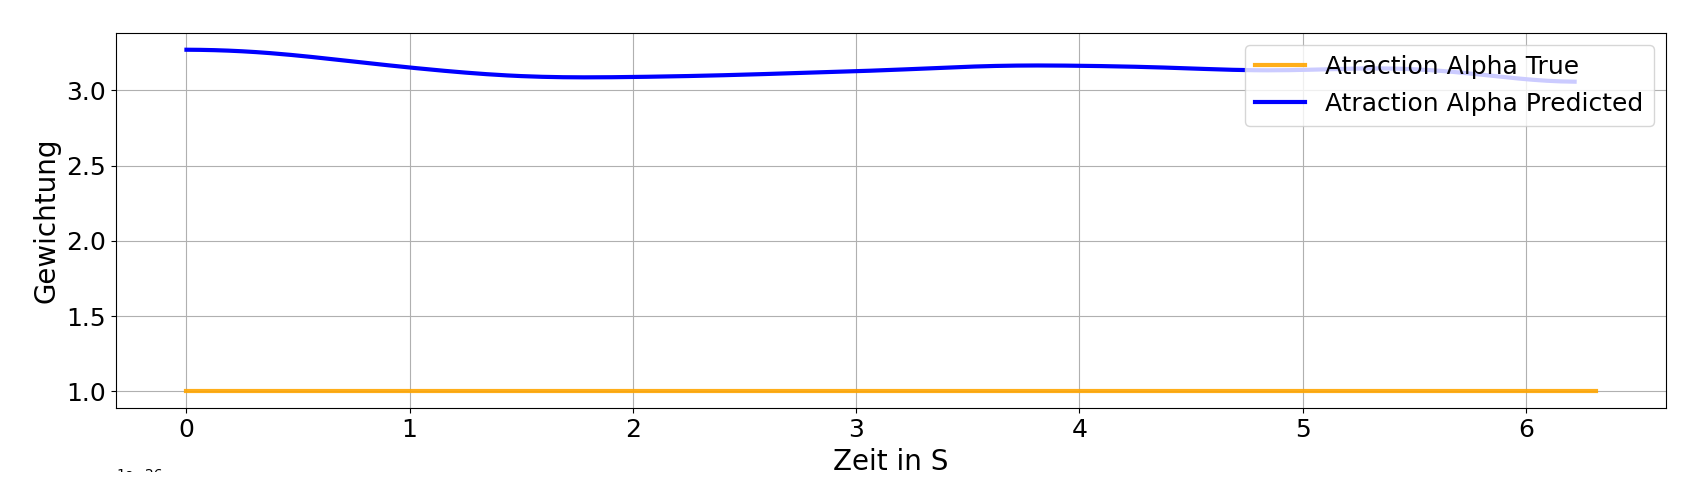
\includegraphics[width=1.0\textwidth]{figures/Experimente/10Fisch/PWD_alpha3.png} 
\end{tabular}
\caption{Parameter $\alpha_3$ für das eigene Modell \label{fig:PWD_Alpha3}}
\end{figure}

Abbildungen \ref{fig:PWD_Alpha1} - \ref{fig:PWD_Alpha3} zeigen, dass auch hier die Parameter recht konstant vorhergesagt wurden, jedoch in allen drei Fällen mit einem zu hohen Wert. Aus Abschnitt \ref{sec:eigenesModell} geht jedoch hervor, dass die Parameter nur Skalierungsfaktoren sind. Teilt man die Alphas durch 3 und multipliziert das Gamma mit 3, so erhält man in etwa die korrekten Parameter.


\begin{figure}[H]
\centering
\begin{tabular}{cc}
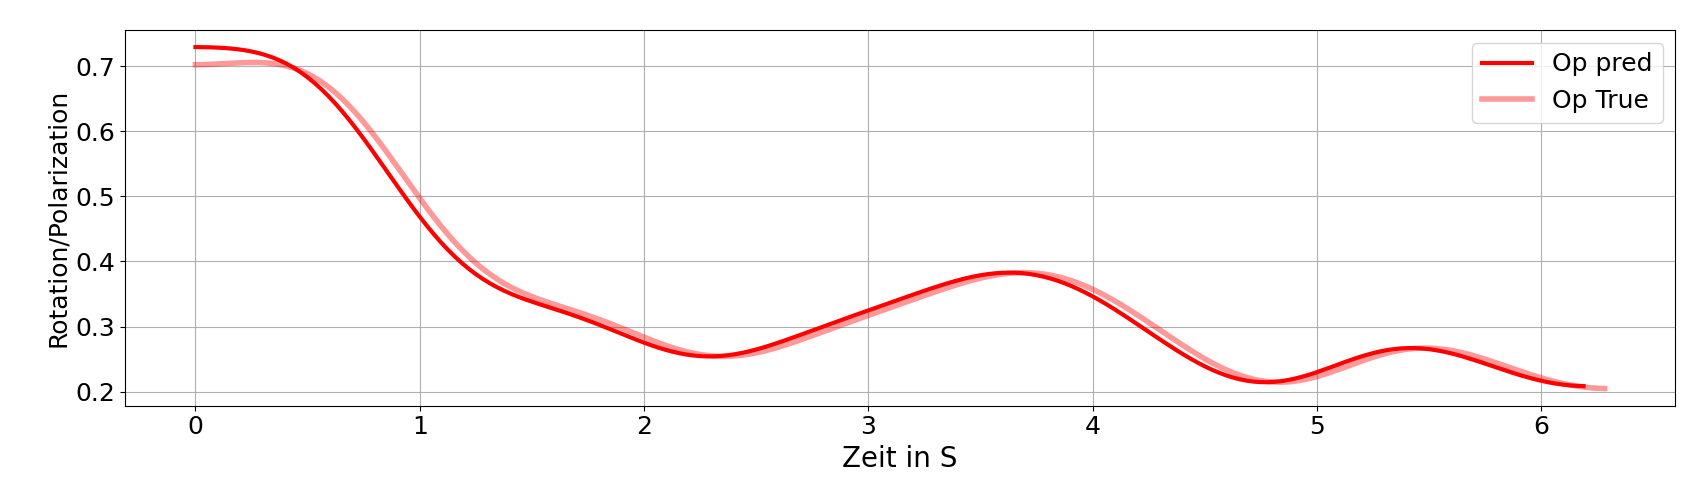
\includegraphics[width=1.0\textwidth]{figures/Experimente/10Fisch/PWD_Pol.png} 
\end{tabular}
\caption{Polarisierungszustand für das eigene Modell \label{fig:PWD_Pol}}
\end{figure}

\begin{figure}[H]
\centering
\begin{tabular}{cc}
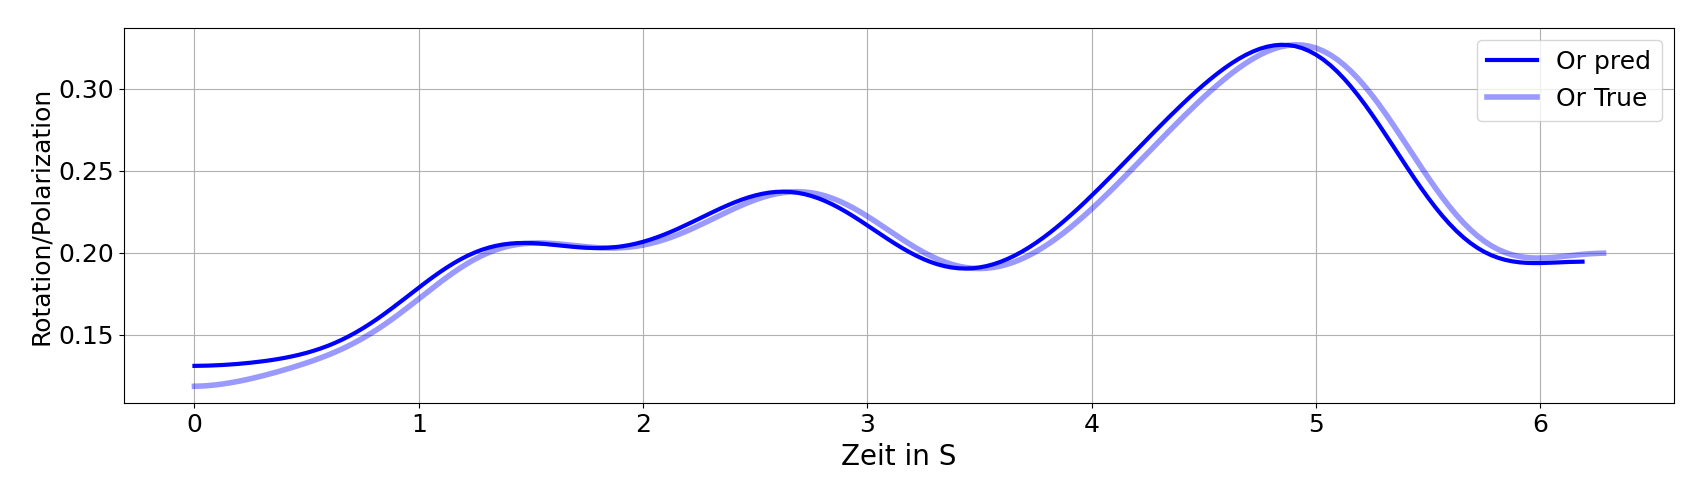
\includegraphics[width=1.0\textwidth]{figures/Experimente/10Fisch/PWD_Rot.png} 
\end{tabular}
\caption{Rotationszustand für das eigene Modell \label{fig:PWD_Rot}}
\end{figure}

Ein Blick auf die Schwarmzustände zeigt auch hier, dass die Rotation und Polarisation für die künstlich erzeugten Daten und die der Approximation übereinstimmen.

\begin{figure}[H]
\centering
\begin{tabular}{cc}
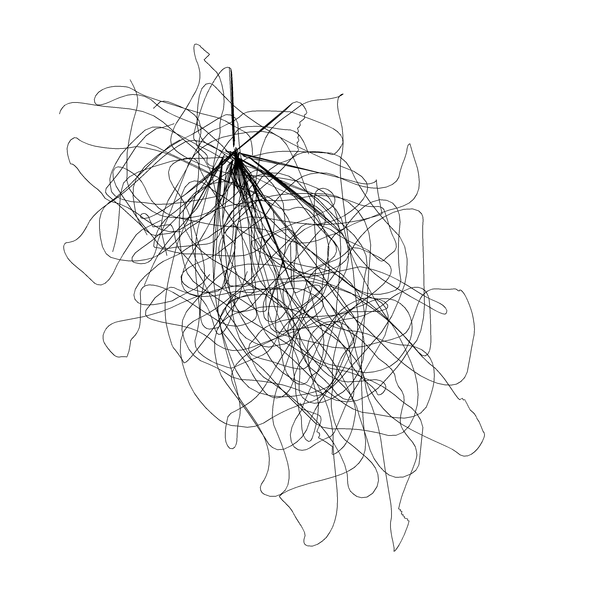
\includegraphics[width=0.5\textwidth]{figures/Experimente/10Fisch/pwd_true.png}&
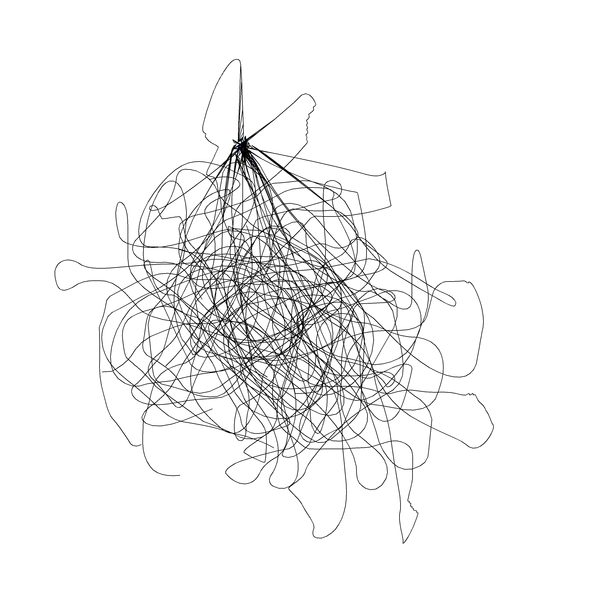
\includegraphics[width=0.5\textwidth]{figures/Experimente/10Fisch/pwd_pred.png}
\end{tabular}
\caption{Trajektorien der künstlich erzeugten Daten (links) und der mittels approximierten Parametern (rechts) \label{fig:APWD}}
\end{figure}

In Abbildung \ref{fig:APWD} sind die Trajektorien von diesem Teil des Experimentes zu sehen. Es sind durchaus Laufwege zu erkennen, die in beiden Graphen die gleichen sind. Allerdings existieren in beiden Graphen auch Laufwege, die in den jeweils anderen Graphen nicht vorhanden sind.

\subsection{Diskussion}

Die Parameterapproximation für konstante Parameter anhand von künstlichen Daten funktioniert für beide Modelle.
Die Erkenntnis, die aus diesem Teil der Arbeit gezogen werden kann, ist, dass aus verschiedenen Parametersets dasselbe Verhalten erreicht werden kann. Anhand des erreichten Fehlers ist zu erkennen, dass RMD für die Approximation zuverlässig funktioniert.
PSO minimiert den Fehler zwar, allerdings schwankt der Fehler für das metrische Boids Modell stark und weicht häufig von null ab.
Im Mittel funktioniert die Approximation ausreichend gut für beide Modelle. Dies zeigen die Trajektorien, die sich in beiden Fällen sehr ähnlich sind sowie die Zustandsdiagramme, für die das Gleiche gilt.


\subsection{Approximierung von variablen Parametern}

In diesem Abschnitt wird die Approximation von Parametern anhand von künstlichen erzeugten Daten untersucht.
Den Agenten werden wie in Abschnitt \ref{AVKP} zufällige Startpositionen und Richtungsvektoren zugewiesen. Die Simulation wird für einige Sequenzen durchlaufen, wobei zufällig gezogene Parameter das Verhalten der Agenten für die jeweils nächste Sequenz bestimmen.


\subsubsection{Metrisches Boids Modell}

Für dieses Modell wird wie schon zuvor PSO verwendet. Die Anzahl der Partikel pro Dimension ist hierbei 50.
Nach maximal 300 Iterationen wird die Suche nach Parametern abgebrochen.

\begin{figure}[H]
\centering
\begin{tabular}{cc}
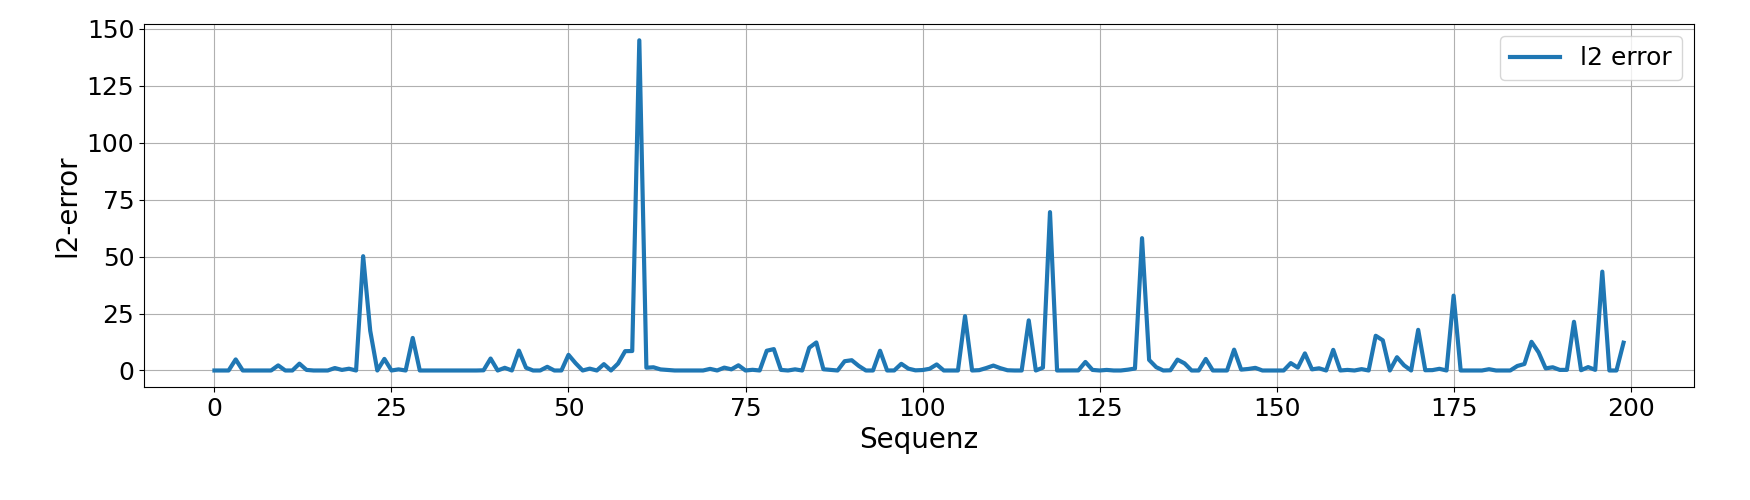
\includegraphics[width=1.0\textwidth]{figures/Experimente/Parameter_variabel/Boids_l2.png} 
\end{tabular}
\caption{L2 Fehler für das Boids Modell mit variablen Parametern \label{fig:Boids_PV_l2}}
\end{figure}

In obiger Abbildung ist der Fehler pro Sequenz zu sehen. Im Vergleich zum Fehler für die Approximation von konstanten Parametern (siehe Abbildung \ref{fig:l2errorBoids10FischeStatisch}) ist zu erkennen, dass hier der Fehler im Mittel geringer ausfällt.
Die maximalen Spitzenwerte fallen jedoch höher aus. Da konstante Parameter eine geringere Herausforderung darstellen sollten, ist hier jedoch zu erwarten, dass der Fehler im Mittel höher ausfällt. Die Erklärung liefert hier die Arbeitsweise von PSO. Die zufällige Platzierung der Partikel im Suchraum ist ein treibender Faktor. Dazu kommt, dass nicht nur die Platzierung vom Zufall abhängt, sondern auch das Aktualisieren der Positionen der Partikel. Hieraus resultieren unterschiedliche Ergebnisse für die Parameterapproximationen. Insbesondere bedeutet das, dass beim mehrfachen Durchlauf desselben Experiments unterschiedliche Parameter und Fehler als Resultat auftreten.
\begin{figure}[H]
\centering
\begin{tabular}{cc}
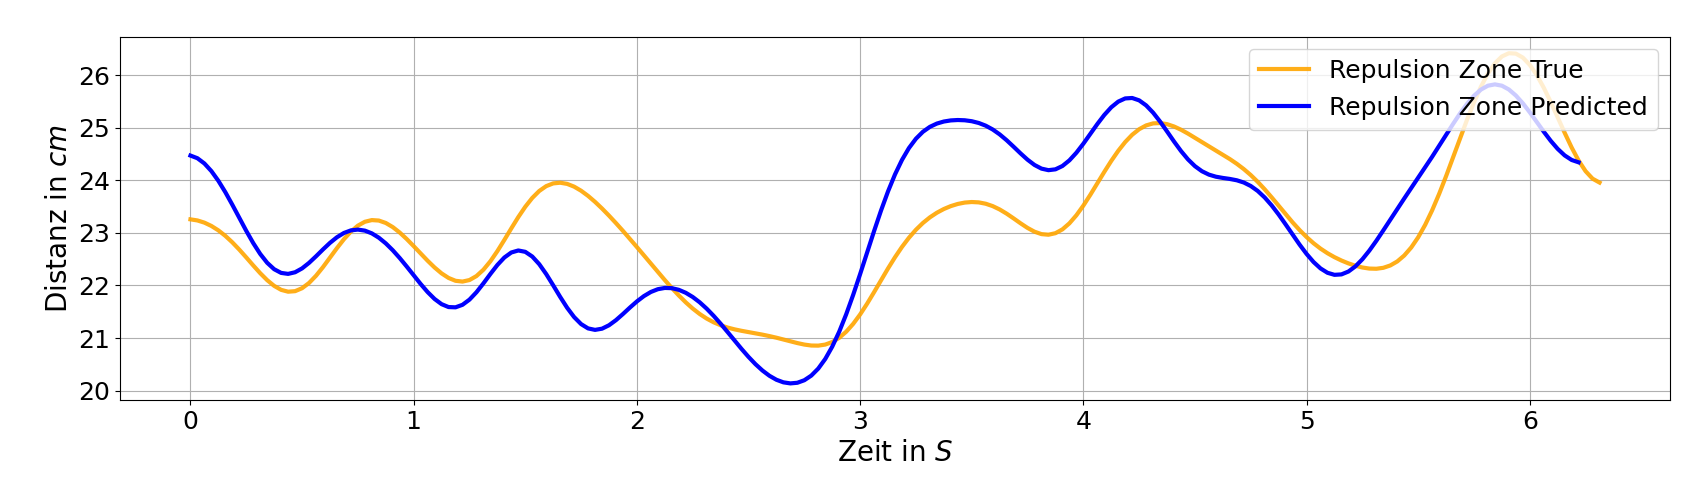
\includegraphics[width=1.0\textwidth]{figures/Experimente/Parameter_variabel/Boids_R.png} 
\end{tabular}
\caption{Abstandhalten Zone für das metrische Boids Modell mit variablen Parametern  \label{fig:Boids_PV_R}}
\end{figure}

\begin{figure}[H]
\centering
\begin{tabular}{cc}
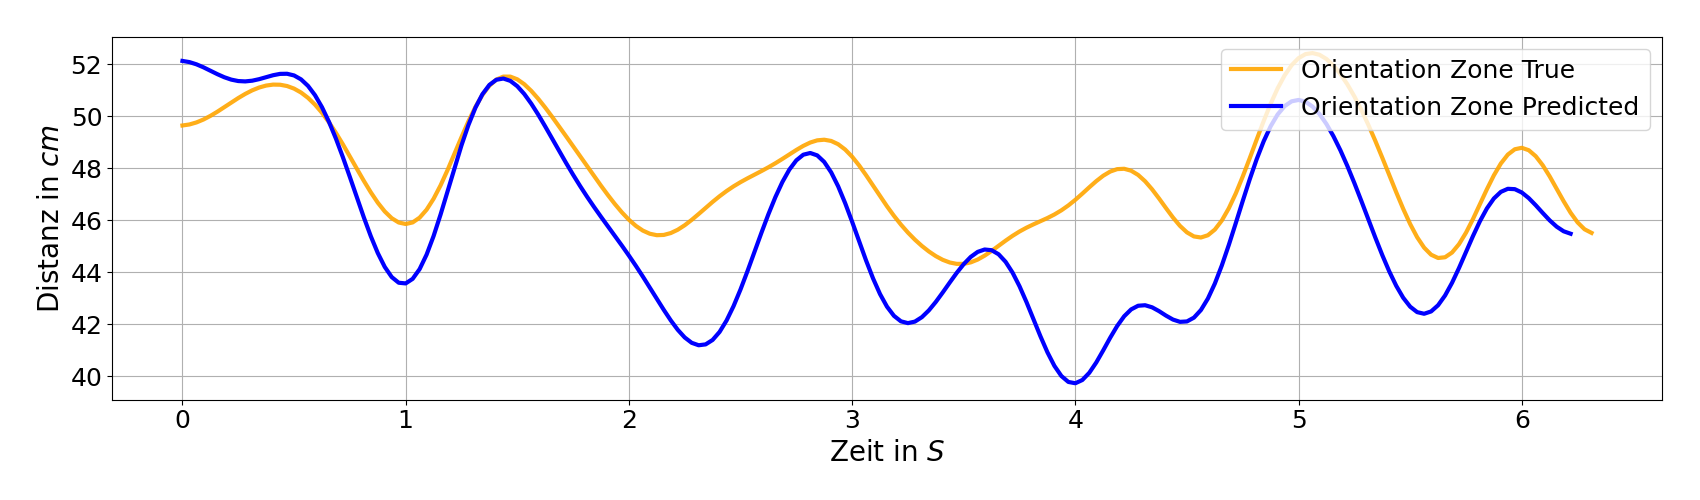
\includegraphics[width=1.0\textwidth]{figures/Experimente/Parameter_variabel/Boids_O.png} 
\end{tabular}
\caption{Orientierungszone für das metrische Boids Modell mit variablen Parametern \label{fig:Boids_PV_O}}
\end{figure}

\begin{figure}[H]
\centering
\begin{tabular}{cc}
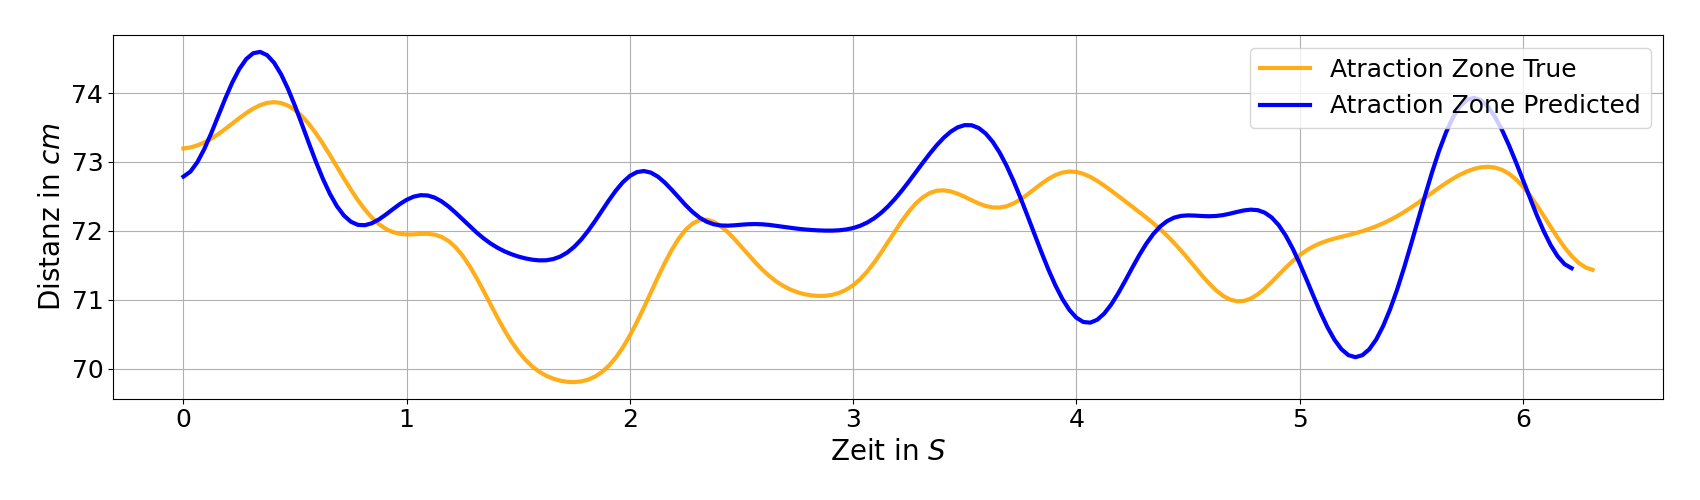
\includegraphics[width=1.0\textwidth]{figures/Experimente/Parameter_variabel/Boids_A.png} 
\end{tabular}
\caption{Attraktionszone für das metrische Boids Modell mit variablen Parametern \label{fig:Boids_PV_A}}
\end{figure}

Die Vorhersage der Parameter für die drei Zonen ist in den Abbildungen \ref{fig:Boids_PV_R} - \ref{fig:Boids_PV_A} in Blau dargestellt, die der korrekten Werte in Gelb. Zu sehen ist, dass die Parameter sich über die Zeit hinweg verändern.
Die Vorhersage ist hierbei relativ nahe bei den korrekten Werten. Die höchste Diskrepanz von ca. 8 cm befindet sich bei der Orientierungszone zum Zeitpunkt 4 Sekunden. Zudem kann man erkennen, dass die Zonen sich nicht überlappen. Das hat zur Folge, dass jede Zone relevant ist.

\begin{figure}[H]
\centering
\begin{tabular}{cc}
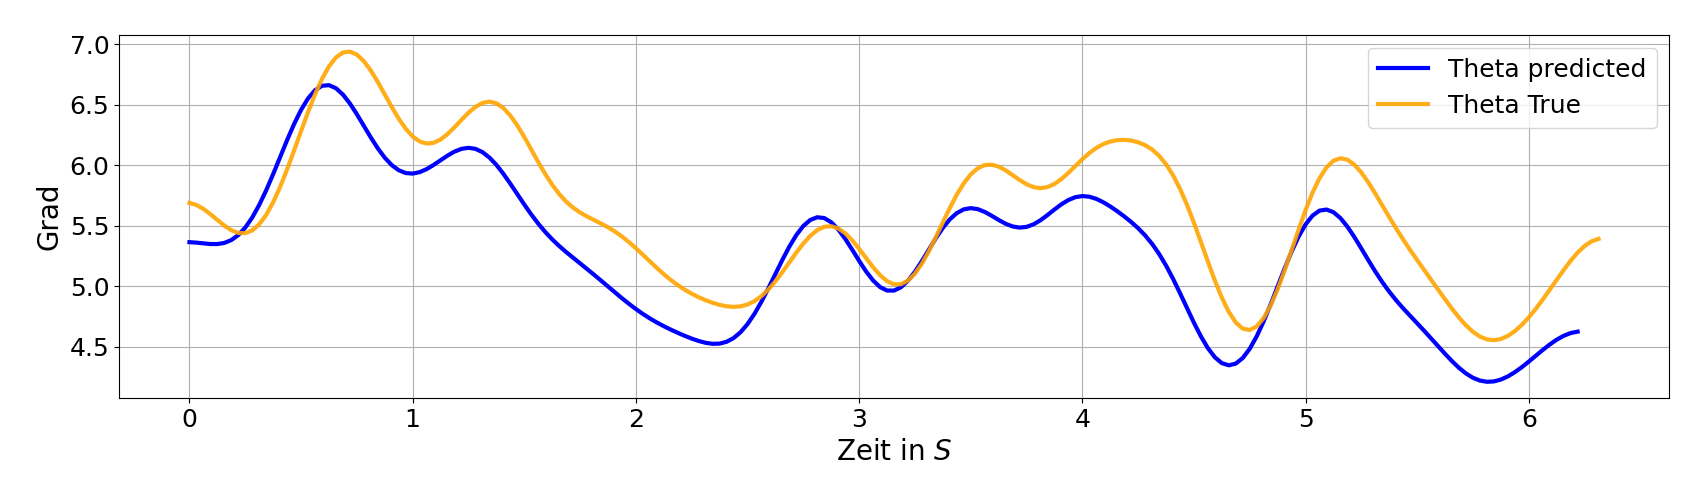
\includegraphics[width=1.0\textwidth]{figures/Experimente/Parameter_variabel/Boids_T.png} 
\end{tabular}
\caption{Einschlagwinkel für das metrische Boids Modell mit variablen Parametern \label{fig:Boids_PV_T}}
\end{figure}

Der Einschlagwinkel ist in Abbildung \ref{fig:Boids_PV_T} dargestellt. Hier ist zu sehen, dass der Verlauf der Kurven sehr ähnlich ist. Die Verschiebung in Y-Richtung beträgt nicht mehr als 0.5 Grad. 

\begin{figure}[H]
\centering
\begin{tabular}{cc}
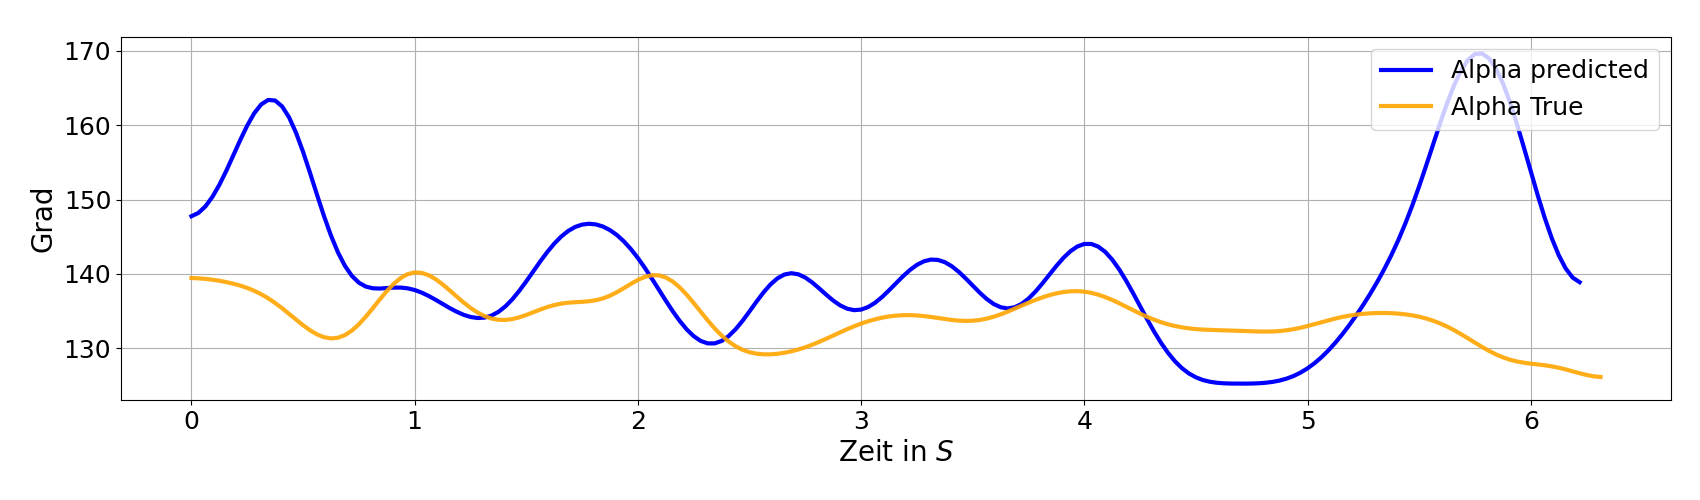
\includegraphics[width=1.0\textwidth]{figures/Experimente/Parameter_variabel/Boids_Alpha.png} 
\end{tabular}
\caption{Blinde Zone für das metrische Boids Modell mit variablen Parametern \label{fig:Boids_PV_Alpha}}
\end{figure}

Der Winkel der blinden Zone der künstlichen Daten und dessen Vorhersage ist in Abbildung \ref{fig:Boids_PV_Alpha} zu sehen.
Der größte Unterschied ist mit um die 30 Grad kurz vor Sekunde 6 zu sehen. Ansonsten verlaufen die Kurven eher unähnlich aber nahe beieinander. Die Relevanz der blinden Zone ist wie die anderen Zonen abhängig davon ob sich Agenten darin befinden.



\begin{figure}[H]
\centering
\begin{tabular}{cc}
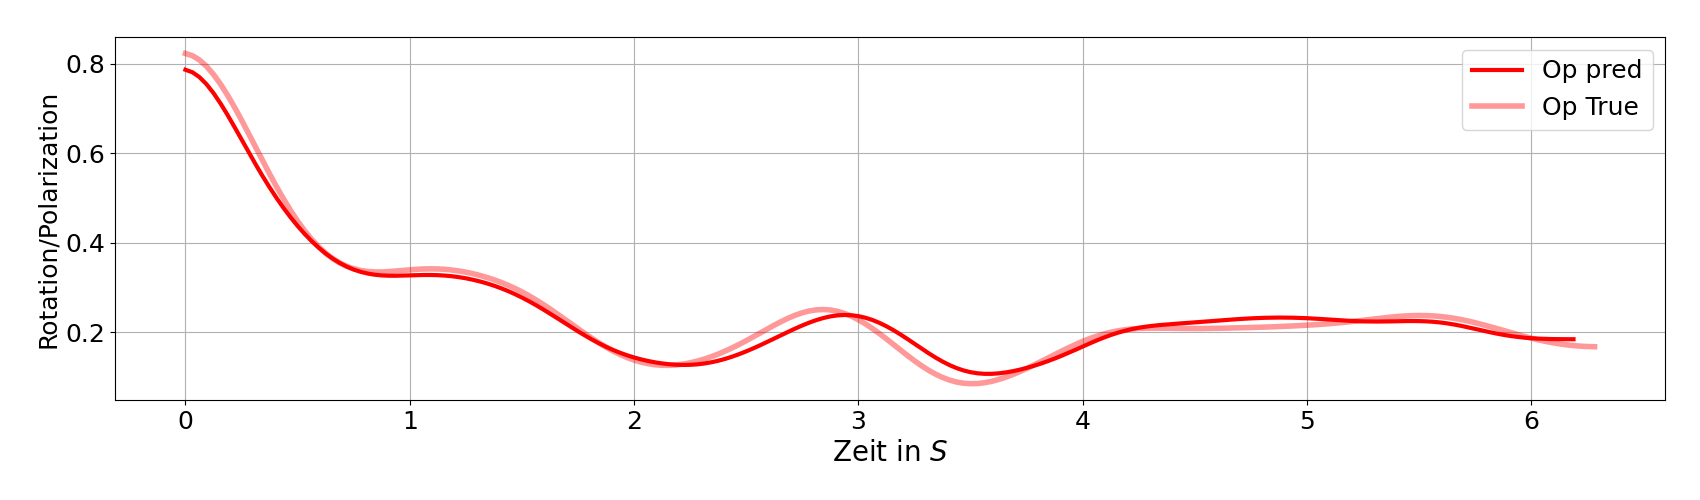
\includegraphics[width=1.0\textwidth]{figures/Experimente/Parameter_variabel/Boids_POL.png} 
\end{tabular}
\caption{Zustand der Polarisierung für das Boids Modell mit variablen Parametern \label{fig:Boids_PV_POL}}
\end{figure}

Der Zustand der Polarisierung ist in obiger Abbildung zu sehen. Der Verlauf der Kurve ist fast identisch und daher kann hieraus geschlossen werden, dass das Verhalten der Agenten im Bezug auf die Polarisierung auch nahe beieinander liegt.

\begin{figure}[H]
\centering
\begin{tabular}{cc}
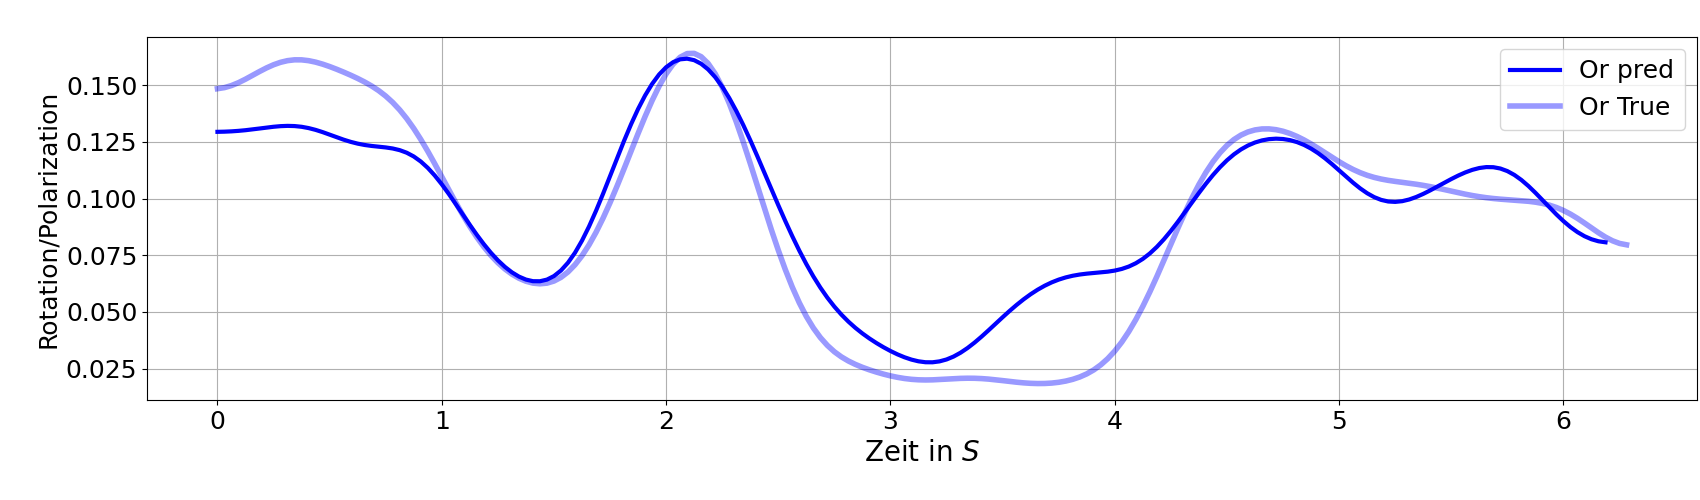
\includegraphics[width=1.0\textwidth]{figures/Experimente/Parameter_variabel/Boids_ROT.png} 
\end{tabular}
\caption{Rotationszustand für das Boids Modell mit variablen Parametern \label{fig:Boids_PV_ROT}}
\end{figure}
Die Kurven für den Rotationszustand verlaufen relativ nahe beieinander. Anzumerken ist, dass der Wertebereich sehr niedrig ist und somit keine Rotation vorhanden ist.


\begin{figure}[H]
\centering
\begin{tabular}{cc}
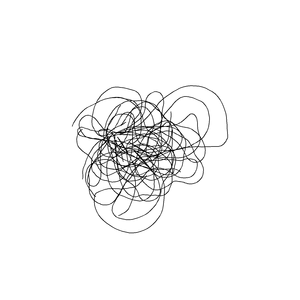
\includegraphics[width=0.5\textwidth]{figures/Experimente/Parameter_variabel/Boids_sim_fake.png}&
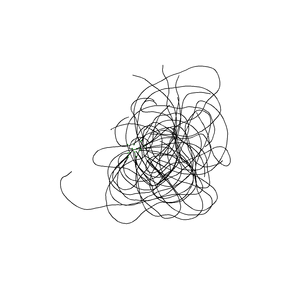
\includegraphics[width=0.5\textwidth]{figures/Experimente/Parameter_variabel/Boids_sim_fake1.png}
\end{tabular}
\caption{Trajektorien der künstlich erzeugten Daten (links) und der mittels approximierten Parametern (rechts) \label{fig:AP}}
\end{figure}

Auch hier ist wieder zu sehen, dass die Laufwege des Boids Modells nicht identisch sind. Die Trajektorien sind deutlich zu unterscheiden, ihr Verlauf ist dennoch ähnlich. Die Agenten bewegen sich in diesem Fall recht gleichmäßig im Raum.
Es gibt keine Position, die von den Agenten ungewöhnlich oft besucht wird. Man kann wie auch schon zuvor erkennen, dass der Zusammenhalt gegeben ist.

\subsubsection{Eigenes Modell}

Für das eigene Modell wird auch hier RMD genutzt mit der Lernrate 0.02 und ADAM zur Anpassung der Lernrate.
Die Suche nach Parametern läuft für 2000 Iterationen.

\begin{figure}[H]
\centering
\begin{tabular}{cc}
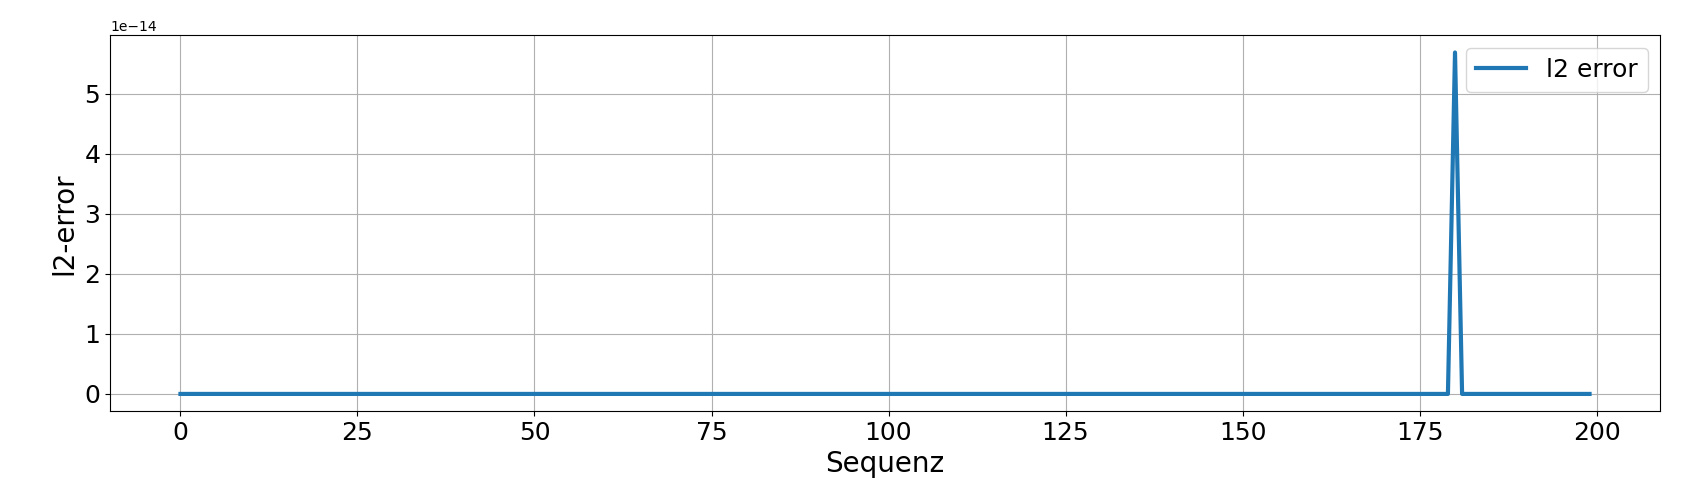
\includegraphics[width=1.0\textwidth]{figures/Experimente/Parameter_variabel/PWD_l2.png} 
\end{tabular}
\caption{L2-Fehler für das eigene Modell mit variablen Parametern  \label{fig:PWD_PV_l2}}
\end{figure}

Der Fehler für das eigene Modell ist hier ebenfalls niedriger als für das metrische Boids Modell.
Der maximale Wert liegt hier bei $5e^{-14}$ was gleich null entspricht. Auch hier kann man sehen, dass die Approximation via RMD einen geringen Fehler produziert.
\begin{figure}[H]
\centering
\begin{tabular}{cc}
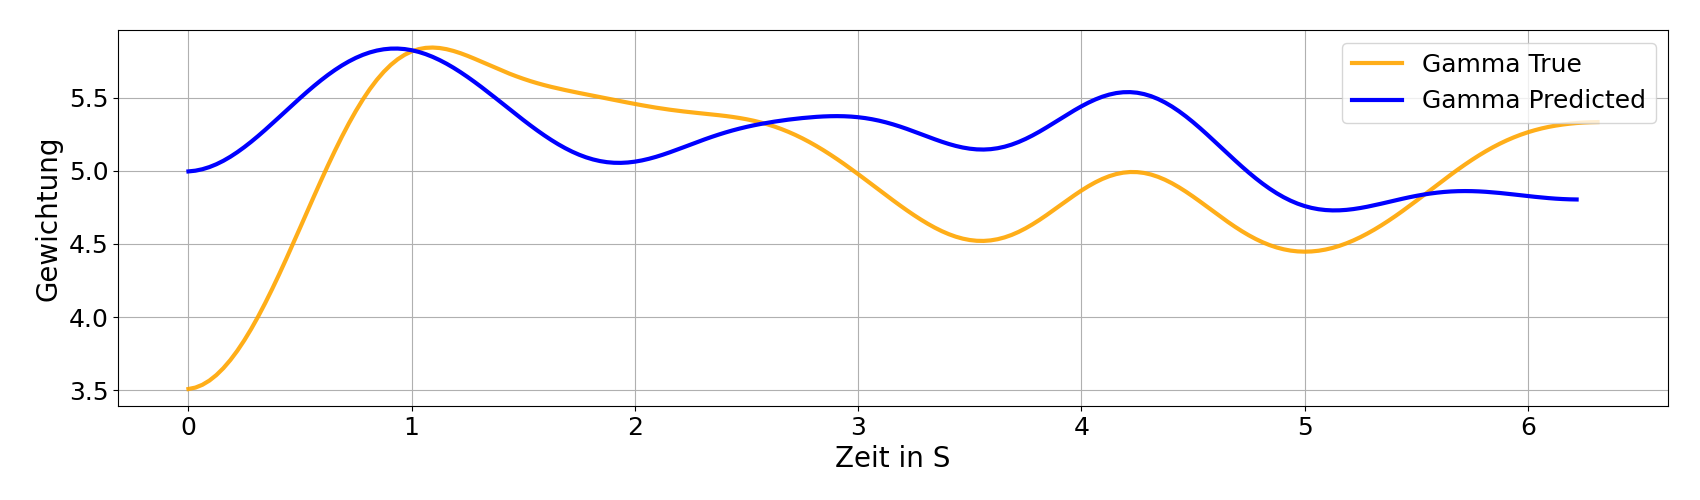
\includegraphics[width=1.0\textwidth]{figures/Experimente/Parameter_variabel/PWD_Gamma.png} 
\end{tabular}
\caption{Parameter $\gamma$ des eigenen Modells mit variablen Parametern \label{fig:PWD_PV_Gamma}}
\end{figure}

Die Approximation des Gammawertes zeigt, dass die Vorhersage relativ nahe bei dem korrekten Gammawert liegt.

\begin{figure}[H]
\centering
\begin{tabular}{cc}
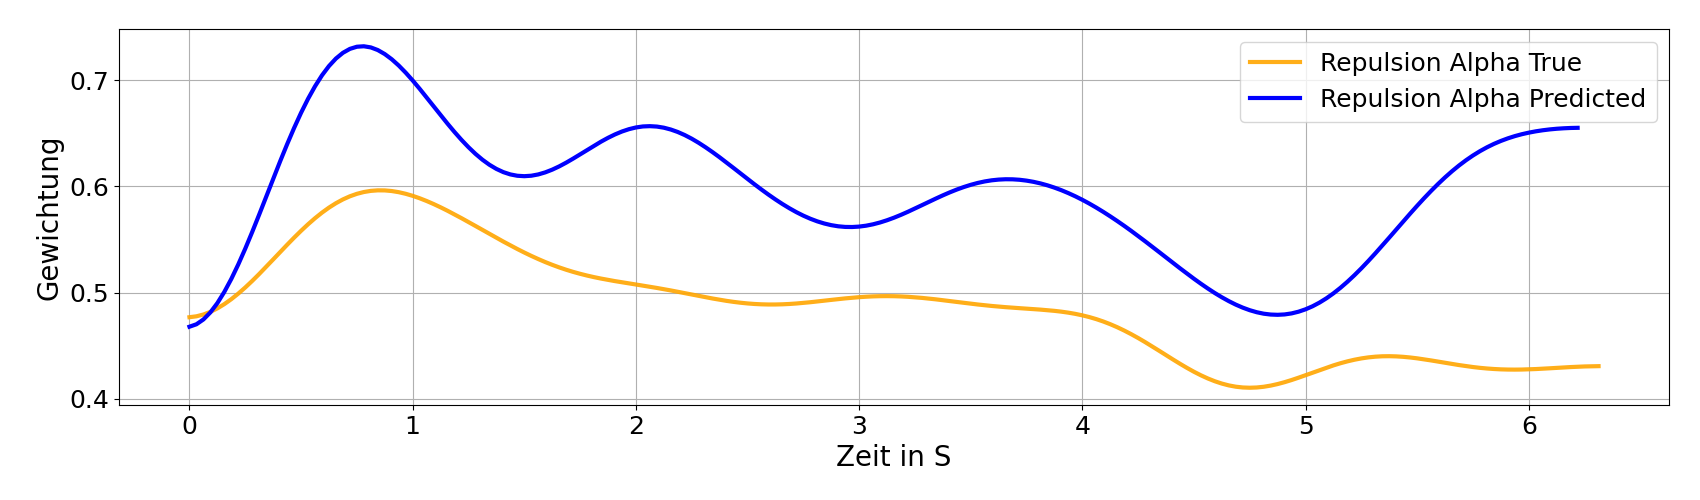
\includegraphics[width=1.0\textwidth]{figures/Experimente/Parameter_variabel/PWD_R.png} 
\end{tabular}
\caption{Parameter $\alpha_1$  des eigenen Modells mit variablen Parametern \label{fig:PWD_PV_R}}
\end{figure}

\begin{figure}[H]
\centering
\begin{tabular}{cc}
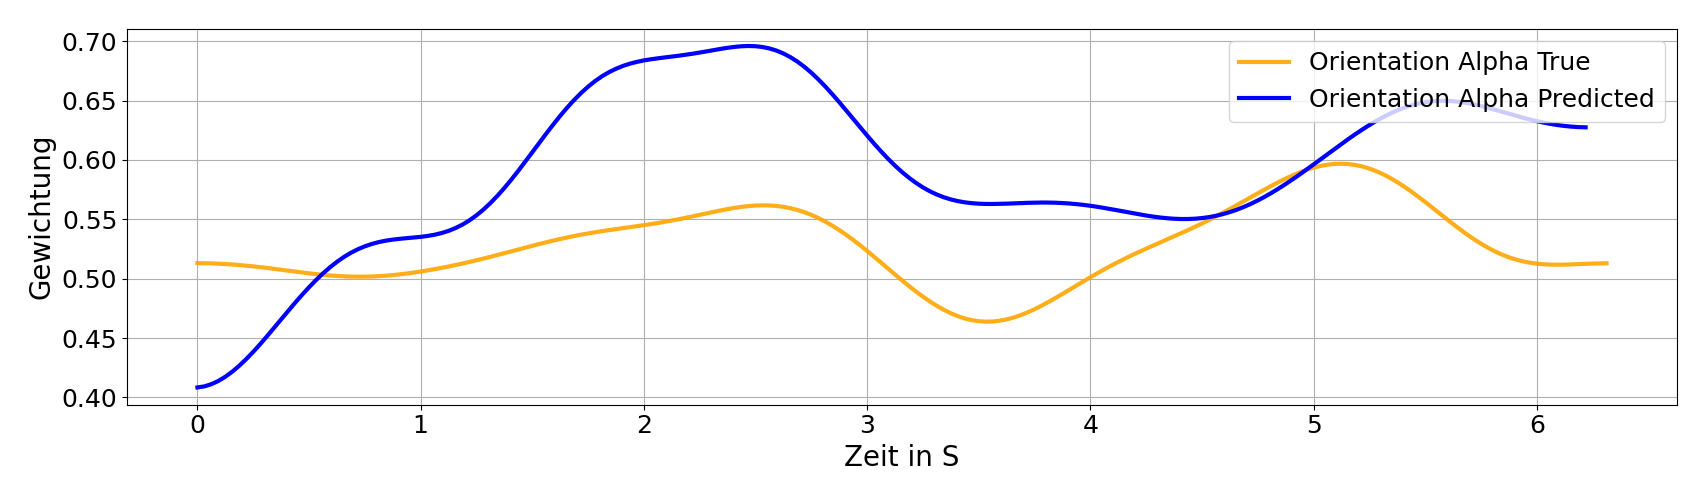
\includegraphics[width=1.0\textwidth]{figures/Experimente/Parameter_variabel/PWD_O.png} 
\end{tabular}
\caption{Parameter $\alpha_2$  des eigenen Modells mit variablen Parametern \label{fig:PWD_PV_O}}
\end{figure}

\begin{figure}[H]
\centering
\begin{tabular}{cc}
\includegraphics[width=1.0\textwidth]{figures/Experimente/Parameter_variabel/PWD_A.png} 
\end{tabular}
\caption{Parameter $\alpha_3$  des eigenen Modells mit variablen Parametern \label{fig:PWD_PV_A}}
\end{figure}

Die Alphaparameter, wie sie in den oberen drei Abbildungen zu sehen sind, zeigen einen jeweils unterschiedlichen Kurvenverlauf.
Auch hier liegen diese nahe beieinander. Wie zuvor erwähnt, sind die Alphaparameter und der Gammaparameter Skalierungsfaktoren, wodurch unterschiedliche Parameterkonstellationen das gleiche Verhalten für die Simulation bedeuten können.
\begin{figure}[H]
\centering
\begin{tabular}{cc}
\includegraphics[width=1.0\textwidth]{figures/Experimente/Parameter_variabel/PWD_POL.png} 
\end{tabular}
\caption{Polarisierungszustand für das eigene Modell mit variablen Parametern \label{fig:PWD_PV_POL}}
\end{figure}

Die Polarisierungszustände der künstlichen Daten und der Approximation liegen hier auch sehr nahe beieinander.
Zu Beginn lässt sich ein Unterschied feststellen, der in etwa bei $0.03$ liegt.

\begin{figure}[H]
\centering
\begin{tabular}{cc}
\includegraphics[width=1.0\textwidth]{figures/Experimente/Parameter_variabel/PWD_ROT.png} 
\end{tabular}
\caption{Rotationszustand für das eigene Modell mit variablen Parametern\label{fig:PWD_PV_ROT}}
\end{figure}

Der Rotationszustand liegt auch für variable Parameter nahe beieinander. Auch hier kann nur zu Beginn ein Unterschied festgestellt werden, der bei ca $0.02$ liegt.

\begin{figure}[H]
\centering
\begin{tabular}{cc}
\includegraphics[width=0.5\textwidth]{figures/Experimente/Parameter_variabel/pwd_true.png}&
\includegraphics[width=0.5\textwidth]{figures/Experimente/Parameter_variabel/pwd_pred.png}
\end{tabular}
\caption{Trajektorien der künstlich erzeugten Daten (links) und der mittels approximierten Parametern (rechts) \label{fig:APWD}}
\end{figure}

Die Pfade der Agenten sind hier ebenfalls sehr ähnlich. Es lässt sich erkennen, dass die Agenten einen recht starken Drang zum Mittelpunkt haben. Im Vergleich zum Modell von Boids sind die Pfade hier und auch schon im Experiment zuvor recht scharfkantig.
Das metrische Boids Modell zeichnet sich durch einen geradlinigen Verlauf der Pfade aus. Der entscheidende Faktor ist hierbei der Einschlagswinkel, der in diesem Modell nicht vorhanden ist.

\subsection{Diskussion}

Die Approximation für die variablen Parameter zeigt für beide Modelle, dass die Zustände der Schwärme ähnlich verlaufen.
Die exakten Parameter wurden für beide Modelle nicht erreicht. Die Zustandsverläufe sind trotzdem sehr nahe beieinander.
Es lässt sich zu diesem Zeitpunkt vermuten, dass eine Parameterbestimmung für die realen Trajektorien der Fische zu bewältigen ist.
Zu erwarten ist, dass die Approximation anhand der Realdaten unterschiedliche Trajektorien zustande kommen. Das eigene Modell wird eher zentrierte Pfadwege besitzen mit durchaus kantigen Pfaden. Das metrische Boids Modell hingegen wird einen gleichmäßigen Verlauf aufweisen.

Ein Rotationszustand oder Polarisationszustand stellte sich mit den zufällig gezogenen Parametern nicht ein.
Es gilt nun zu ergründen, ob die Zustände der realen Daten von den Modellen abgebildet werden können.

\section{Approximation anhand von realen Daten}

Die vorherigen Experimente haben gezeigt, dass aus der Approximation der Parameter für künstliche Daten Parameter resultieren, welche dieselben Zustände erzeugten können wir die der Simulation. In diesem Teil des Kapitels werden Parameter anhand der Trajektorien aus Abschnitt \ref{ab:EDD} der Fischschwärme approximiert. Dazu werden die beiden vorgestellten Modelle begutachtet.

 Als Kostenfunktion wurde wie schon zuvor die l2-Kostenfunktion verwendet. Die nachfolgenden Bilder zeigen den Fehler über einen Zeitraum von 2000 Bildsequenzen, was in etwa 65 Sekunden entspricht. Die betrachtete Schwarmgröße beträgt 10 Fische wobei für beide Modelle dieselben Sequenzen approximiert werden.

\begin{figure}[H]
\centering
\begin{tabular}{cc}
\includegraphics[width=1.0\textwidth]{figures/Experimente/Realdaten/Boidsl2Fehler_10Fische.png} \\
\includegraphics[width=1.0\textwidth]{figures/Experimente/Realdaten/PWD2Fehler_10Fische.png}  
\end{tabular}
\caption{Kostenfunktion für das metrische Boids Modell (oben) und das eigene Modell (unten)\label{fig:10Fisch}}
\end{figure}

Beim betrachten des Fehlers erkennt man, dass der Fehler des metrischen Boids Modells die ersten 1000 Sequenzen stark ansteigt und bei ca. $5e^{-7}$ sein Maximum findet. Nach dem Maximum sinkt der Fehler wieder ab, bleibt jedoch in einem relativ hohen Wertebereich. Der Fehler des eigenen Modells hat sein Maximum bei $1250$ und ist insgesamt in einem niedrigeren Wertebereich als der des metrischen Modells. Hieraus kann man schließen, dass das eigene Modell für die Parameterapproximation anhand von Realdaten besser geeignet ist als das metrische Boids Modell. Ein Blick auf die Zustände bestätigt diese Beobachtung.

\begin{figure}[H]
\centering
\begin{tabular}{cc}
\includegraphics[width=1.0\textwidth]{figures/Experimente/Realdaten/Boids_10F_zust_Pol.png} 
\end{tabular}
\caption{Kostenfunktion für das metrische Boids Modell (oben) und das eigene Modell (unten)\label{fig:10Fisch_boids_Pol}}
\end{figure}

Der Zustand der Polarisierung des Schwarms und der Simulation mit approximierten Parametern unterscheiden sich sehr stark.
Das Modell zeigt keine Polarisierung, da dessen Wertebereich nahezu durchgehend unter $0.65$ liegt. Die Realdaten hingegen weisen in einigen Bereichen Polarisierung auf. Beispielsweise liegt der Wertebereich der Polarisierung für die Realdaten zwischen Sekunde $40$ und $45$ bei mehr als $0.65$ und der Wertebereich der Rotation bei unter $0.35$.

\begin{figure}[H]
\centering
\begin{tabular}{cc}
\includegraphics[width=1.0\textwidth]{figures/Experimente/Realdaten/Boids_10F_zust_Rot.png} 
\end{tabular}
\caption{Rotationszustand der Realdaten mit 10 Fischen und des metrische Boids Modells\label{fig:10Fisch_rot_boids}}
\end{figure}

Auch der Rotationszustand, wie er in Abbildung \ref{fig:10Fisch_rot_boids} zu sehen ist zeigt, dass dieser von der Simulation nicht abgebildet wird. Zwar ist der Wertebereich näher beieinander, jedoch kann kein ähnlicher Verlauf ausgemacht werden.
Hierbei findet Rotation der Realdaten ausschließlich in den ersten $1-4$ Sekunden statt.
Die nachfolgende Abbildung zeigt die Zustandsverläufe für das eigene Modell.

\begin{figure}[H]
\centering
\begin{tabular}{cc}
\includegraphics[width=1.0\textwidth]{figures/Experimente/Realdaten/PWD_10F_zust.png} 
\end{tabular}
\caption{Polarisationszustand (oben) und Rotationszustand (unten) des eigenen Modells und des Schwarms der größe 10 Fische\label{fig:10Fisch}}
\end{figure}

Zu erkennen ist, dass in beiden Fällen die Kurven sehr ähnlich verlaufen. Wie zuvor beschrieben findet Polarisation innerhalb der Realdaten statt. Somit kann das Modell Polarisation abbilden. Das Abbilden der Rotation ist hier nicht eindeutig zu sehen. Wie in Abschnitt \ref{ab:EDD} dargelegt, neigen die kleineren Schwärme weniger zur Rotation als die großen Schwärme. Demzufolge wird hierfür später ein größerer Schwarm betrachtet.

\begin{figure}[H]
\centering
\begin{tabular}{ccc}
\includegraphics[width=0.33\textwidth]{figures/Experimente/Realdaten/Boids_10_Fisch_real.png} &
\includegraphics[width=0.33\textwidth]{figures/Experimente/Realdaten/Boids_10_Fisch.png} &
\includegraphics[width=0.33\textwidth]{figures/Experimente/Realdaten/PWD_10_Fisch.png} 
\end{tabular}
\caption{Trajektorien der Realdaten für 10 Fische (links), des metrischen Boids Modells (mitte) und des eigenen Modells (rechts)\label{fig:10Fisch}}
\end{figure}

Abbildung \ref{fig:10Fisch} zeigt die Trajektorien der Realdaten und der Modelle. Es ist festzustellen, dass die drei Trajektorien sehr unterschiedlich sind. Der echte Schwarm schwimmt kreisförmig um ein Zentrum herum. 

Die Simulation des Boids Modells zeigt keine eindeutige Strukturierung.Ich frag mal frau bub Zu sehen ist, dass sich ein Agent komplett vom Schwarm entfernt. Die restlichen Agenten bleiben beieinander, entfernen sich jedoch nicht weit von ihrer Ausgangsposition.

Die Simulation des eigenen Modells zeigt eine Struktur, welche Zusammenhalt aufweist. Die Agenten haben einen starken Drang zur Mitte, werden allerdings immer wieder nach außen getrieben. Es findet ein Expandieren und Kollabieren der Struktur statt.


Nun stellt sich die Frage, wieso die Trajektorien der Realdaten keinen Rotationszustand erreichen, wenn diese doch eine eindeutige Rotation aufweist. Der Schwarm ist durch den Versuchsaufbau gezwungen, im Kreis zu schwimmen. Dadurch werden die Fische über eine längere Zeit eine Kreisbewegung ausführen. Das Rotationsdiagramm hingegen entsteht durch die Orientierung der Fische einer Momentaufnahme. Demnach kann die Orientierung der Fische in einem Moment eine schwache Ausprägung der Rotation besitzen, was über die Zeit hinweg dennoch in einer Rotation resultiert.

Das nachfolgende Experiment wird mit den Trajektorien von $60$ Fischen durchgeführt, wobei diese eine stärkere Rotation aufweisen werden. Hierbei werden wie zuvor 2000 Sequenzen durchlaufen, was in etwa 65 Sekunden entspricht.


\begin{figure}[H]
\centering
\begin{tabular}{cc}
\includegraphics[width=1.0\textwidth]{figures/Experimente/Realdaten/Boidsl2Fehler_60Fische.png} \\
\includegraphics[width=1.0\textwidth]{figures/Experimente/Realdaten/PWD2Fehler_60Fische.png}  
\end{tabular}
\caption{Kostenfunktion für das metrische Boids Modell (oben) und das eigene Modell (unten)\label{fig:60Fisch}}
\end{figure}

Auch hier ist wieder ein großer Unterschied bezüglich der Kosten zu sehen. Das Maximum der Kosten für das metrische Modell liegt bei $2e^{8}$ im Vergleich dazu liegt das Maximum des eigenen Models bei $2e^{5}$ und somit um den Faktor $1000$ niedriger. Die Kosten des eigenen Modells sind im Durchschnitt fünfstellig, die des Modells von Boids weitestgehend achtstellig (bis auf die ersten Sequenzen). Die Zustandsdiagramme zeigen ein ähnliches Verhalten wie die Diagramme für den kleineren Schwarm.

\begin{figure}[H]
\centering
\begin{tabular}{cc}
\includegraphics[width=1.0\textwidth]{figures/Experimente/Realdaten/Boids_60F_zust_Pol.png} 
\end{tabular}
\caption{Rotationszustand der Realdaten mit 60 Fischen und des metrische Boids Modells\label{fig:60Fisch_pol_boids}}
\end{figure}

Wie Abbildung \ref{fig:60Fisch_rot_boids} zeigt, passt sich die Kurve nicht der des Datensatzes an. Sie verläuft weitestgehend linear. Daraus kann man schließen, dass die Agenten der Simulation in unterschiedliche Richtungen schwimmen. Da so gut wie keine Polarisation stattfindet, kann auch keine Rotation stattfinden. Um zu rotieren, müssen die Agenten in gewisser Weiße gleichgerichtet sein. Dies ist nur der Fall, wenn die Agenten gemeinsam in eine Richtung schwimmen. Dies zeigt das nächste Diagramm.

\begin{figure}[H]
\centering
\begin{tabular}{cc}
\includegraphics[width=1.0\textwidth]{figures/Experimente/Realdaten/Boids_60F_zust_Rot.png} 
\end{tabular}
\caption{Rotationszustand der Realdaten mit 60 Fischen und des metrische Boids Modells\label{fig:60Fisch_rot_boids}}
\end{figure}

Auch hier findet bei der Simulation keinerlei Rotation statt (der Anfang sei ausgenommen). Die Trajektorien der Realdaten (transparent) zeigen hier jedoch eine deutliche Rotation. Vom Zeitpunkt $0$ bis ca. $10$ Sekunden ist $Or > 0.65$ und $Op < 0.35$ (Siehe Abbildung \ref{fig:60Fisch_pol_boids}). Auch hier bildet das Modell das Verhalten der Realdaten nicht ab.

Das eigene Modell zeigt auch für eine größere Anzahl an Fischen ein ähnliches Verhalten wie für den kleineren Schwarm.

\begin{figure}[H]
\centering
\begin{tabular}{cc}
\includegraphics[width=1.0\textwidth]{figures/Experimente/Realdaten/PWD_60Fische_POL.png} 
\end{tabular}
\caption{Polarisationszustand der Realdaten mit 60 Fischen und des eigenen Modells\label{fig:60Fisch_pol_EIGEN}}
\end{figure}

Auch hier liegen die Kurven nahe beieinander. Wie beim kleineren Schwarm sind die Unterschiede hier marginal.

\begin{figure}[H]
\centering
\begin{tabular}{cc}
\includegraphics[width=1.0\textwidth]{figures/Experimente/Realdaten/PWD_60Fische_ROT.png} 
\end{tabular}
\caption{Rotationszustand der Realdaten mit 60 Fischen und des eigenen Modells\label{fig:60Fisch_rot_EIGEN}}
\end{figure}

Gleiches gilt für den Rotationszustand, wie er oben zusehen ist. Auch hier lässt sich feststellen, dass das Modell die Zustände gut imitiert.

Ein Blick auf die Trajektorien zeigt die verschiedenen Verhaltensmuster der Daten und der Simulation.

\begin{figure}[H]
\centering
\begin{tabular}{ccc}
\includegraphics[width=0.33\textwidth]{figures/Experimente/Realdaten/Fisch_60_REAL.png} &
\includegraphics[width=0.33\textwidth]{figures/Experimente/Realdaten/Boids_60_Fisch.png} &
\includegraphics[width=0.33\textwidth]{figures/Experimente/Realdaten/PWD_60_Fisch_sim.png} 
\end{tabular}
\caption{Trajektorien der Realdaten für 60 Fische (links), des metrischen Boids Modells (mitte) und des eigenen Modells (rechts)\label{fig:60FischTraj}}
\end{figure}

In der Abbildung \ref{fig:60FischTraj} sind links die Trajektorien des Schwarms zusehen. Hier lässt sich feststellen, dass der Schwarm wie auch zuvor rotiert. Die Wege der Fische sind relativ ausgeglichen, wodurch sich die Bahnen gleichmäßig verteilen.
Es existiert somit kein Bereich in dem sich die Fische ungewöhnlich oft aufhalten.

Das metrische Boids Modell ist mittig zu sehen und zeigt auch hier keinerlei Struktur. Die Agenten zeigen keinen Zusammenhalt, was durch die geradlinigen Trajektorien, welche aus dem Bild verschwinden, deutlich wird. Die Agenten sind somit in unterschiedliche Richtungen unterwegs.

Die Simulation für das eigene Modell (rechtes Bild) zeigt wieder die Eigenschaft des Expandieren und des Kollabierens.
Das Zentrum wird von den Agenten häufiger besucht als die Außenbereiche. 

\subsection{Diskussion}

Die Approximation der Parameter für die Modelle zeigt, dass das metrische Boids Modell schon bei den Diagrammen von den Realdaten zu unterscheiden ist. Es lassen sich keine Zustände imitieren und die Pfade der Simulation zeigen keinerlei Ähnlichkeit mit den Realdaten. Der direkte Vergleich der Fehlerfunktion zwischen dem metrischen Boids Modell und dem eigenen Modell zeigt, dass das eigene Modell einen geringeren Fehler pro Sequenz erreicht. Dies zeigt, dass das eigene Modell für die Approximation der Parameter für die Realdaten besser geeignet ist. Ob dies dem Approximierungsverfahren geschuldet ist oder sich das Modell nicht für Realdaten eignet, lässt sich hierbei nicht genau klären. Ein weiterer Kritikpunkt ist, dass kein Gesamtzusammenhalt der Agenten gewährleistet ist. Der Zusammenhalt wird ausschließlich über die Nachbarschaft erreicht. Dies ist ein Problem, wenn ein Agent keine weiteren Agenten in der entsprechenden Zone vorfindet. Daraus resultiert das Herauslösen des Individuums aus dem Schwarm, wie es in diesem Teil der Arbeit zu sehen war.

Das eigene Modell zeigt hinsichtlich der Zustandsdiagramme eine gute Anpassung an die echten Schwarmdaten. Es ist hierbei nicht von diesen zu unterscheiden. Die Trajektorien sprechen hierbei allerdings eine andere Sprache. Die Fische der echten Daten schwimmen in relativ ausgeglichner Weiße im Becken und bevorzugen keinen Bereich. Die Agenten der Simulation des eigenen Modells bevorzugen das Massezentrum, welches durch die Gesamtheit der Agenten entsteht. Dies ist somit deren bevorzugter Aufenthaltsbereich und unterscheidet hiermit die Realdaten von den simulierten Daten. Teilt man einem Leihen mit, dass sich Fischschwärme in ausgeglichener Art durch das Wasser bewegen, so wird dieser anhand der Trajektorien sofort die Realdaten von den simulierten unterscheiden können.

Dass die Agenten des eigenen Modells zum Mittelpunkt getrieben werden, ist der Gewichtungsfunktion (siehe Abschnitt \ref{sec:eigenesModell}) geschuldet. Dies gewährleistet zum einen den Zusammenhalt der Individuen, zum anderen werden die Agenten wie ein Gummiband zurück zum Massezentrum getrieben, je stärker diese sich vom Zentrum entfernen. Es bräuchte eine Kraft die dem entgegenwirkt um eine stabile Rotation zu erreichen.
% chapter experimente (end)